% Necoyoad Architecture Blueprint
% An extensive reverse-engineered software architecture paper
% based on the public database dump at github.com/yosietserga/necoyoad

\documentclass[11pt,a4paper]{article}

% ============================================================
%  Packages
% ============================================================
\usepackage[T1]{fontenc}
\usepackage[utf8]{inputenc}
\usepackage{lmodern}
\usepackage{microtype}

\usepackage{graphicx}
\usepackage{xcolor}
\usepackage{geometry}
\usepackage{amsmath}
\usepackage{amssymb}

\usepackage{tcolorbox}
\tcbuselibrary{skins,breakable,listings}
\usepackage{colortbl}
\usepackage{booktabs}
\usepackage{tabularx}
\usepackage{longtable}
\usepackage{array}
\usepackage{enumitem}
\usepackage{adjustbox}
\usepackage{caption}
\captionsetup{justification=raggedright, singlelinecheck=false, font=small, labelfont=bf}
\usepackage{fancyhdr}
\usepackage{titlesec}
\usepackage{pdflscape}

% TikZ for diagrams
\usepackage{tikz}
\usetikzlibrary{arrows.meta,positioning,calc,shapes.geometric,fit,backgrounds,chains,decorations.pathreplacing,shapes.multipart}

% hyperref - load last among content packages
\usepackage[
    colorlinks=true,
    linkcolor=blue!50!black,
    citecolor=blue!40!black,
    urlcolor=blue!60!black,
    bookmarks=true,
    bookmarksnumbered=true,
    unicode=true,
    pdftitle={Necoyoad --- Software Architecture Blueprint},
    pdfauthor={Reverse-Engineered Architecture Report},
    pdfsubject={Software Architecture, Database Schema Analysis, OpenCart-derived CMS},
    pdfkeywords={Necoyoad, OpenCart, PHP, MySQL, MyISAM, CMS, E-Commerce, EAV, Multi-Store, Polymorphic Associations}
]{hyperref}

% ============================================================
%  Page geometry
% ============================================================
\geometry{a4paper, top=2.4cm, bottom=2.4cm, left=2.4cm, right=2.4cm}
\setlength{\headheight}{14pt}

% ============================================================
%  Headings / header-footer
% ============================================================
\pagestyle{fancy}
\fancyhf{}
\fancyhead[L]{\small\itshape Necoyoad Architecture Blueprint}
\fancyfoot[C]{\small\thepage}
\renewcommand{\headrulewidth}{0.3pt}
\renewcommand{\footrulewidth}{0pt}

\titleformat{\section}{\Large\bfseries\color{black!85}}{\thesection}{0.6em}{}
\titleformat{\subsection}{\large\bfseries\color{black!80}}{\thesubsection}{0.6em}{}
\titleformat{\subsubsection}{\normalsize\bfseries\color{black!75}}{\thesubsubsection}{0.5em}{}

% Orphans/widows
\widowpenalty=10000
\clubpenalty=10000

% Give LaTeX more flexibility to break lines (prevents overfull hboxes
% in narrow columns and in tcolorbox \texttt{} listings).
\emergencystretch=4em
\hbadness=10000
\hfuzz=2pt
\vfuzz=2pt

% Allow sloppy line breaking globally (helps with consecutive \texttt{} tokens)
\sloppy

% ============================================================
%  Custom colors for diagrams
% ============================================================
\definecolor{necoyoad-blue}{HTML}{1F4E79}
\definecolor{necoyoad-orange}{HTML}{B85C00}
\definecolor{necoyoad-green}{HTML}{2E6B33}
\definecolor{necoyoad-purple}{HTML}{5B2A86}
\definecolor{nodefill}{HTML}{F4F7FB}
\definecolor{nodefillalt}{HTML}{FBF4EE}
\definecolor{nodefillgreen}{HTML}{F2F8F2}
\definecolor{nodefillpurple}{HTML}{F5EFFA}
\definecolor{nodefillgray}{HTML}{F0F0F2}
\definecolor{accent}{HTML}{1F4E79}
\definecolor{softgray}{HTML}{6E6E6E}

% tcolorbox styles
\newtcolorbox{infobox}[1][]{
  enhanced, breakable,
  colback=nodefill, colframe=necoyoad-blue!60,
  boxrule=0.4pt, arc=2pt, left=8pt, right=8pt, top=6pt, bottom=6pt,
  fonttitle=\bfseries\small, coltitle=white,
  title=#1
}
\newtcolorbox{warningbox}[1][]{
  enhanced, breakable,
  colback=nodefillalt, colframe=necoyoad-orange!70,
  boxrule=0.4pt, arc=2pt, left=8pt, right=8pt, top=6pt, bottom=6pt,
  fonttitle=\bfseries\small, coltitle=white,
  title=#1
}

% ============================================================
%  Document
% ============================================================
\begin{document}

% No title page in the body. The cover is rendered separately via
% HTML/Playwright (Template 04 scholarly dark) and merged as page 0.

\thispagestyle{empty}

% ------------------------------------------------------------
% Abstract
% ------------------------------------------------------------
\begin{center}
{\Large\bfseries Necoyoad --- A Reverse-Engineered Software Architecture Blueprint}\\[0.4em]
{\small\itshape An extensive, diagram-rich reconstruction of a legacy PHP/MySQL\\
multi-store e-commerce and content platform}\\[1.2em]
\end{center}

\begin{abstract}
\noindent
This document is a verbose, deeply detailed blueprint of the \textbf{Necoyoad} web
application, a custom PHP/MySQL platform that the author (\textit{yosietserga})
published as a single phpMyAdmin database dump on GitHub in February 2023. The
repository under analysis contains no application source code; only the
\texttt{necoyoad\_db.sql} dump is present. We therefore reconstruct the runtime
architecture, the domain model, the cross-cutting patterns and the inferred
user-facing flows by treating the 87-table relational schema as the primary,
and largely sufficient, source of truth.

The reconstruction shows a system whose design vocabulary is clearly inherited
from the OpenCart 1.x/2.x lineage (table names, the \texttt{product\_to\_category}
junction style, the \texttt{url\_alias} SEO layer, the
\texttt{order\_total} extension point, the
\texttt{customer\_group} pricing model) but extended far beyond a vanilla store
with: (i) a polymorphic object graph (\texttt{object},
\texttt{object\_to\_category}, \texttt{object\_to\_store},
\texttt{description}, \texttt{property}, \texttt{status},
\texttt{url\_alias}) that acts as a typed Entity-Attribute-Value (EAV) spine;
(ii) a full content-management surface (\texttt{post}, \texttt{menu},
\texttt{banner}, \texttt{widget}, \texttt{theme}, \texttt{template},
\texttt{theme\_style}); (iii) a marketing/CRM surface
(\texttt{newsletter}, \texttt{campaign}, \texttt{contact},
\texttt{contact\_list}, \texttt{campaign\_contact}, \texttt{campaign\_link},
\texttt{campaign\_stat}, \texttt{campaign\_link\_stat}); (iv) a Venezuelan-style
bank-transfer payment surface (\texttt{bank}, \texttt{bank\_account},
\texttt{order\_payment}, \texttt{balance}); (v) a warehouse inventory surface
(\texttt{warehouse\_movement}); and (vi) a self-hosted task scheduler
(\texttt{task}, \texttt{task\_queue}, \texttt{task\_exec}) that drives
the marketing campaigns.

We deliberately \emph{do not} improve, modernise or recommend changes. The
goal of the paper is purely descriptive: a faithful, exhaustive map of the
system as it was the morning of 3 February 2023, the timestamp frozen into the
dump header. Eighteen TikZ diagrams, six inventory tables and an
appendix listing every one of the 87 tables accompany the prose.
\end{abstract}

\vspace{0.6em}
\noindent\textbf{Keywords:} Necoyoad, OpenCart lineage, PHP 8.1, MySQL 5.7,
MyISAM, phpMyAdmin dump, EAV, polymorphic associations, multi-store, multi-language,
MVC, front controller, task scheduler, bank-transfer payments, CMS,
marketing campaigns, SEO URL aliases.

\newpage

% ------------------------------------------------------------
\tableofcontents
\newpage

% ============================================================
\section{Introduction}\label{sec:intro}
% ============================================================

\subsection{Subject of the Blueprint}

\textbf{Necoyoad} is the public-facing name of a custom web application whose
only publicly-published artifact is a phpMyAdmin database dump committed to
GitHub by the user \texttt{yosietserga} under the repository
\href{https://github.com/yosietserga/necoyoad}{\texttt{github.com/yosietserga/necoyoad}}.
The repository is, in the strictest sense, a single-file repository: it contains
exactly one commit (``Add files via upload''), one branch (\texttt{main}), and
one file --- \texttt{necoyoad\_db.sql}. There is no \texttt{README}, no
license file, no \texttt{composer.json}, no \texttt{.htaccess}, no PHP source
whatsoever. The application code itself is, at the time of writing, not
publicly available.

This paper treats the SQL dump as a forensic snapshot of the application's
data layer and reconstructs, from that snapshot, the surrounding architecture
that must have produced it. Database schemas carry a surprisingly large amount
of architectural intent: every foreign-key column declares a dependency, every
\texttt{enum} or \texttt{status} column declares a state machine, every
\texttt{date\_added} / \texttt{date\_modified} pair declares an audit
expectation, every polymorphic pair \texttt{(object\_id, object\_type)}
declares an indirection point. Eighty-seven tables, taken together, are more
than enough to reverse-engineer a coherent picture of the runtime.

\subsection{Scope and Stance}

The reader should treat this document as an \emph{architecture blueprint},
not a tutorial, a review, or a refactoring proposal. Three rules govern the
text below:

\begin{enumerate}[leftmargin=1.6em,itemsep=2pt]
  \item \textbf{Descriptive, not prescriptive.} We document what the system
        \emph{is}. We do not propose changes, modernisations, or ``best-practice''
        rewrites. Where a design choice looks unusual from a 2023-vantage
        point (for example, the use of the MyISAM engine, or the absence of
        declared foreign keys), we describe the consequences and leave it
        there.
  \item \textbf{Inference clearly labelled.} Where the schema directly tells
        us something, we state it as fact. Where we are inferring behaviour
        that the schema only implies (for example, the precise lifecycle of
        an order, or the exact routing algorithm), we say so explicitly and
        justify the inference.
  \item \textbf{Diagrams over prose where possible.} The eighteen TikZ figures
        are the spine of the document. They are designed to be readable on
        their own; the surrounding prose exists to explain, contextualise and
        cross-reference them, not to substitute for them.
\end{enumerate}

\subsection{Document Roadmap}

Section~\ref{sec:provenance} catalogues the artifact itself: the dump file,
its metadata, the table prefix, the engine choices, the charset choices, the
collation choices. Section~\ref{sec:stack} reconstructs the runtime stack
(PHP/Apache or Nginx/MySQL/phpMyAdmin) that the dump's header advertises.
Section~\ref{sec:style} identifies the architectural style as an
OpenCart-derived Model-View-Controller (MVC) with several custom extensions,
and introduces the four cross-cutting patterns (polymorphic object graph,
EAV-style descriptions, multi-store scoping, multi-language scoping) that
recur throughout the schema.

Section~\ref{sec:schema} is the longest. It walks through every functional
domain --- catalog, customers, orders, payments, banking, marketing, CMS,
inventory, tax/geo, themes, tasks, users, stats, settings --- and draws an
Entity-Relationship diagram (ERD) for each. Section~\ref{sec:crosscutting}
extracts the patterns that span domains. Sections~\ref{sec:lifecycle}
through~\ref{sec:cron} reconstruct three runtime lifecycles (an HTTP request,
a customer checkout, a task-scheduler tick). Sections~\ref{sec:seo}
through~\ref{sec:security} cover SEO/URL routing, the audit trail and the
security/permission model. Section~\ref{sec:integrity} discusses the
data-integrity consequences of the MyISAM/no-foreign-keys choice.
Section~\ref{sec:observations} closes with non-recommendatory observations.
Appendix~\ref{app:inventory} lists all 87 tables in a single long table for
reference; Appendix~\ref{app:polymorphic} enumerates every polymorphic
association in the schema.

% ============================================================
\section{Provenance and Artifact Description}\label{sec:provenance}
% ============================================================

\subsection{The Repository}

\begin{table}[htbp]
\centering
\caption{Repository and artifact provenance.}\label{tab:provenance}
\small
\begin{tabularx}{\columnwidth}{lX}
\toprule
\textbf{Field} & \textbf{Value} \\
\midrule
Repository URL & \url{https://github.com/yosietserga/necoyoad} \\
Owner          & \texttt{yosietserga} \\
Default branch & \texttt{main} \\
Total commits  & 1 (``Add files via upload'') \\
Files in repo  & 1 (\texttt{necoyoad\_db.sql}, 76\,467 bytes) \\
License        & None declared \\
README         & None \\
Source code    & None --- database dump only \\
\bottomrule
\end{tabularx}
\end{table}

\subsection{The Dump File Header}

The SQL file begins with a phpMyAdmin banner. The banner is more than
ceremony: it pins down, with no ambiguity, the exact server configuration
that produced the dump, and therefore the configuration against which the
schema was, at minimum, known to compile. The relevant lines are reproduced
verbatim below.

\begin{tcolorbox}[enhanced,colback=nodefillgray,colframe=black!40,boxrule=0.3pt,arc=2pt,left=8pt,right=8pt,top=4pt,bottom=4pt,fontupper=\small\ttfamily]
-- phpMyAdmin SQL Dump\\
-- version 5.2.0\\
-- https://www.phpmyadmin.net/\\
--\\
-- Host: localhost\\
-- Generation Time: Feb 03, 2023 at 07:37 AM\\
-- Server version: 5.7.17\\
-- PHP Version: 8.1.2
\end{tcolorbox}

\subsection{What the Header Tells Us}

\begin{table}[htbp]
\centering
\caption{Inferred runtime stack from the dump header.}\label{tab:stack}
\small
\begin{tabularx}{\columnwidth}{llX}
\toprule
\textbf{Layer} & \textbf{Version} & \textbf{Implication} \\
\midrule
phpMyAdmin & 5.2.0  & Administrative UI; release date 2022-11-22. \\
MySQL      & 5.7.17 & Released 2016-12; EOL October 2023. \emph{Legacy.} \\
PHP        & 8.1.2  & Released 2021-12; supported at dump time. \\
Host       & localhost & The dump was produced on the same host as the DB. \\
Timezone   & \texttt{+00:00} & Dump taken in UTC; the running app likely uses a different local TZ. \\
SQL mode   & \texttt{NO\_AUTO\_VALUE\_ON\_ZERO} & Inserts of \texttt{0} into AUTO\_INCREMENT columns are preserved (not renumbered). \\
Charset    & \texttt{utf8mb4} (connection) & Full Unicode support at the connection layer. \\
\bottomrule
\end{tabularx}
\end{table}

Two facts deserve emphasis. First, MySQL 5.7 was already in the sunset of
its supported life when the dump was produced (EOL was roughly eight months
away). Second, the dump explicitly sets \texttt{SET FOREIGN\_KEY\_CHECKS=0}
at the top and restores it at the bottom. This is normal phpMyAdmin behaviour,
but it also signals that the schema cannot rely on declared foreign keys for
load-order safety --- which, as Section~\ref{sec:engine} will show, is
moot anyway because the tables are MyISAM and therefore cannot carry
foreign-key constraints at all.

\subsection{Database and Table Prefix}

The database is named \texttt{necoyoad\_db}. Every table is prefixed with
the eight-character random string \texttt{nts8sd4fd\_}; for example,
\texttt{nts8sd4fd\_product}, \texttt{nts8sd4fd\_order},
\texttt{nts8sd4fd\_user}. The prefix is a classic shared-hosting convention:
it lets multiple applications share a single MySQL database without
colliding on common table names like \texttt{user} or \texttt{setting}.
The randomness of the prefix (\texttt{nts8sd4fd}) is mildly defensive ---
it makes the prefix harder to guess in a SQL-injection scenario, although
this is a weak control by modern standards. Throughout this paper we
will drop the prefix when discussing tables in prose (so
``the \texttt{product} table'') but show it in full in code listings and
in the appendix inventory.

\subsection{Engine, Charset and Collation Choices}\label{sec:engine}

Every table in the dump is declared with \texttt{ENGINE=MyISAM}. This is
a consequential choice with several knock-on effects:

\begin{itemize}[leftmargin=1.6em,itemsep=2pt]
  \item \textbf{No foreign keys.} MyISAM does not support
        \texttt{FOREIGN KEY} constraints. All referential integrity is the
        application's responsibility. The schema's many \texttt{\_id}
        columns are therefore \emph{soft} foreign keys --- pointers that
        the database will not enforce.
  \item No transactions. MyISAM is non-transactional; a multi-table write
        (e.g.\ ``insert an order, then insert its line items, then insert
        its totals, then decrement stock'') is not atomic. A crash midway
        leaves the database in a partially-applied state.
  \item Table-level locking. MyISAM locks the whole table for writes,
        which limits concurrency on write-heavy tables (notably
        \texttt{stat}, \texttt{search}, \texttt{user\_activity},
        \texttt{campaign\_stat}, \texttt{campaign\_link\_stat}).
  \item Smaller disk footprint and faster full-table scans than InnoDB,
        which was the historical justification.
\end{itemize}

The charset story is inconsistent in a way that is itself diagnostic. The
\texttt{DEFAULT CHARSET} of most tables is \texttt{latin1}, but individual
columns are frequently overridden to \texttt{CHARACTER SET utf8 COLLATE
utf8\_bin}. This per-column override pattern is exactly what one sees when
an existing latin1 schema has been retrofitted for UTF-8 storage column by
column, rather than migrated wholesale. It is a strong hint that the schema
predates the application's adoption of UTF-8.

The collation \texttt{utf8\_bin} is binary and case-sensitive; this is
unusual for user-facing string columns (which would normally use
\texttt{utf8\_general\_ci} or \texttt{utf8\_unicode\_ci} for
case-insensitive comparison). The choice has subtle consequences: an
\texttt{email} lookup, for instance, would be case-sensitive at the
database level, so the application must normalise email casing in
application code before querying.

\subsection{The 87-Table Inventory at a Glance}

\begin{table}[htbp]
\centering
\caption{Functional domains, table counts and indicative responsibilities.}\label{tab:domains}
\small
\begin{tabularx}{\columnwidth}{lclX}
\toprule
\textbf{\#} & \textbf{Tables} & \textbf{Domain} & \textbf{Indicative responsibility} \\
\midrule
1  & 13 & Catalog / Products    & SKU catalogue, options, attributes, discounts, images, related items, types, manufacturers. \\
2  & 12 & Orders \& Payments    & Order header, line items, totals, history, options, downloads, manual payments, coupons. \\
3  & 8  & Customers \& CRM      & Customer accounts, groups, addresses, wallet balance, reviews, review likes. \\
4  & 9  & Marketing / Campaigns & Newsletters, campaigns, contact lists, per-recipient tracking, link tracking. \\
5  & 4  & Banking               & Bank directory, account numbers, per-order manual transfer payments. \\
6  & 5  & CMS / Content         & Posts, categories, descriptions, banners, banner items. \\
7  & 7  & Presentation          & Menus, menu links, widgets, widget-to-landing-page, templates, themes, theme styles. \\
8  & 3  & Task scheduler        & Task definitions, queue, execution log. \\
9  & 6  & Tax \& Geography      & Countries, zones, geo zones, tax classes, tax rates, zone-to-geo-zone. \\
10 & 4  & Users \& Permissions  & Admin users, user groups, user activity log. \\
11 & 6  & Core polymorphic spine & \texttt{object}, \texttt{object\_to\_category}, \texttt{object\_to\_store}, \texttt{description}, \texttt{property}, \texttt{status}. \\
12 & 5  & Localisation          & Languages, currencies, weight classes, length classes, URL aliases. \\
13 & 4  & Audit \& Analytics    & \texttt{stat}, \texttt{search}, \texttt{notification}, \texttt{review\_likes}. \\
14 & 2  & Settings \& Extensions & \texttt{setting}, \texttt{extension}. \\
15 & 1  & Inventory             & \texttt{warehouse\_movement}. \\
\midrule
   & 87 & \textbf{Total}        & \\
\bottomrule
\end{tabularx}
\end{table}

% ============================================================
\section{Inferred Runtime Stack}\label{sec:stack}
% ============================================================

\subsection{The Apache-or-Nginx / PHP / MySQL Triangle}

The dump header pins MySQL 5.7.17 and PHP 8.1.2. The web server itself is
not named, but two strong signals narrow the choice. First, phpMyAdmin 5.2.0
is installed; phpMyAdmin is overwhelmingly deployed behind Apache with
\texttt{mod\_php}, or behind Nginx with PHP-FPM. Second, the schema's
\texttt{language} table contains a \texttt{directory} column and a
\texttt{filename} column (each language points to a PHP language file on
disk), which is the OpenCart convention and is framework-agnostic.
We can therefore say with confidence that the runtime is some
combination of \{Apache, Nginx\} $\times$ \{mod\_php, PHP-FPM\} $\times$
MySQL 5.7, with PHP 8.1.2 as the interpreter. The exact variant does not
materially affect any of the architectural conclusions below.

\begin{figure}[htbp]
\centering
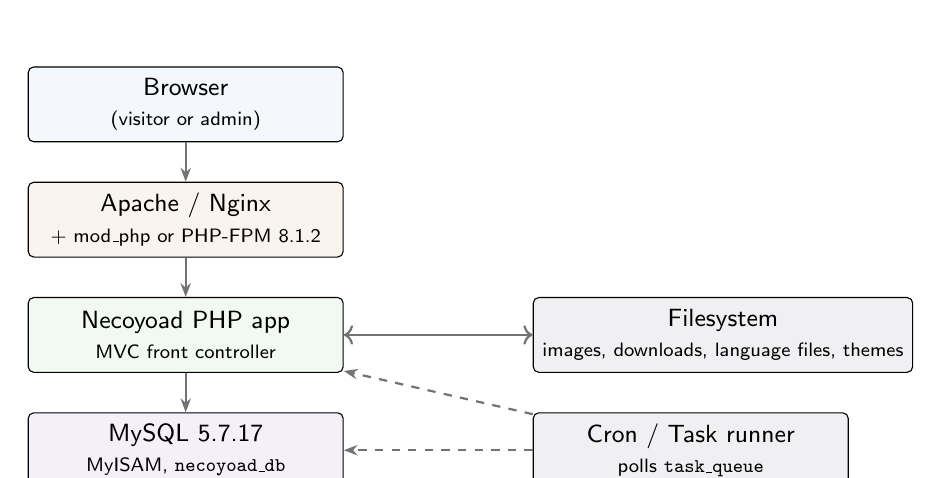
\begin{tikzpicture}[
  layer/.style={draw, rounded corners=2pt, minimum width=4cm,
                minimum height=0.95cm, align=center, font=\small\sffamily},
  arr/.style={-{Stealth[length=5pt]}, thick, black!55}
]
  \node[layer, fill=nodefill]                (browser) {Browser\\\scriptsize (visitor or admin)};
  \node[layer, fill=nodefillalt, below=0.5cm of browser] (web)    {Apache / Nginx\\\scriptsize + mod\_php or PHP-FPM 8.1.2};
  \node[layer, fill=nodefillgreen, below=0.5cm of web]    (php)    {Necoyoad PHP app\\\scriptsize MVC front controller};
  \node[layer, fill=nodefillpurple, below=0.5cm of php]   (db)     {MySQL 5.7.17\\\scriptsize MyISAM, \texttt{necoyoad\_db}};
  \node[layer, fill=nodefillgray, right=2.4cm of php]     (fs)     {Filesystem\\\scriptsize images, downloads, language files, themes};
  \node[layer, fill=nodefillgray, right=2.4cm of db]      (cron)   {Cron / Task runner\\\scriptsize polls \texttt{task\_queue}};
  \draw[arr] (browser) -- (web);
  \draw[arr] (web)     -- (php);
  \draw[arr] (php)     -- (db);
  \draw[arr, <->] (php) -- (fs);
  \draw[arr, dashed] (cron) -- (php);
  \draw[arr, dashed] (cron) -- (db);
\end{tikzpicture}
\caption{Inferred runtime stack. The browser hits the web server,
which dispatches to a PHP process running the Necoyoad MVC application.
The application reads and writes the \texttt{necoyoad\_db} MySQL database
and the filesystem (image uploads, downloadable products, per-language
PHP translation files, theme assets). A separate cron process polls the
\texttt{task\_queue} table and re-enters the application to execute
deferred jobs, primarily the marketing-campaign mailings.}
\label{fig:stack}
\end{figure}

\subsection{Why the Filesystem Still Matters}

Although the dump is database-only, several schema columns tell us that
the filesystem is a first-class data store. The \texttt{language} table
has \texttt{directory} and \texttt{filename} columns; this is the OpenCart
convention of loading \texttt{<directory>/<filename>.php} for translation
strings. The \texttt{download} and \texttt{order\_download} tables store
a \texttt{filename} and a \texttt{mask} --- the mask is what the user sees
when downloading, the filename is the actual on-disk path. The
\texttt{product\_image}, \texttt{manufacturer.image},
\texttt{category.image}, \texttt{banner\_item.image},
\texttt{bank.image}, \texttt{user.image}, \texttt{customer.photo}
columns all hold filesystem paths. The \texttt{store.folder} column
hints that multi-store is implemented by selecting a different
filesystem folder per store. Any complete picture of the application
must include this filesystem half; we will annotate it on each diagram
where it is relevant.

\subsection{Cron or Pseudo-Cron}

The presence of a \texttt{task}, \texttt{task\_queue}, and
\texttt{task\_exec} trio is unambiguous: there is a background job
runner. Whether it is a real Unix \texttt{cron} entry that calls a PHP
CLI script every minute, or a ``pseudo-cron'' triggered by the front
controller on each page load (a common OpenCart-extension pattern), the
schema alone cannot tell us. Section~\ref{sec:cron} discusses both
options. The marketing-campaign subsystem (Section~\ref{sec:marketing})
clearly relies on this scheduler: the \texttt{campaign\_contact}
table has a \texttt{task\_queue\_id} column that ties each
recipient-to-campaign assignment to a queued job.

% ============================================================
\section{Architectural Style and Cross-Cutting Patterns}\label{sec:style}
% ============================================================

\subsection{Style: OpenCart-derived MVC}

The schema's vocabulary is unmistakably OpenCart-derived. The following
table maps OpenCart canonical table names to their Necoyoad counterparts
and notes the divergences.

\begin{table}[htbp]
\centering
\caption{OpenCart-to-Necoyoad table-name mapping (selected).}\label{tab:opencart-mapping}
\footnotesize\sloppy
\begin{tabularx}{\columnwidth}{>{\raggedright\arraybackslash}p{3.6cm}>{\raggedright\arraybackslash}p{3.6cm}X}
\toprule
\textbf{OpenCart (vanilla)} & \textbf{Necoyoad} & \textbf{Divergence} \\
\midrule
\texttt{product}                       & \texttt{product}                       & + \texttt{owner\_id}, \texttt{product\_type}, \texttt{cost} \\
\texttt{product\_description}          & \texttt{description}                   & Generalised to polymorphic \texttt{(object\_id, object\_type)} \\
\texttt{product\_to\_category}         & \texttt{product\_to\_category} + \texttt{object\_to\_category} & Both specific and polymorphic versions exist \\
\texttt{category\_description}         & \texttt{description}                   & Same polymorphic table \\
\texttt{category\_path}                & ---                                    & Not present; categories use \texttt{parent\_id} only \\
\texttt{customer}                      & \texttt{customer}                      & + \texttt{rif}, \texttt{company}, \texttt{photo}, \texttt{birthday}, \texttt{banned}, \texttt{activation\_code} \\
\texttt{order}                         & \texttt{order}                         & + \texttt{rif}, \texttt{coupon\_id} \\
\texttt{order\_total}                  & \texttt{order\_total}                  & identical \\
\texttt{url\_alias}                    & \texttt{url\_alias}                    & + \texttt{object\_id}, \texttt{object\_type} (polymorphic) \\
\texttt{setting}                       & \texttt{setting}                       & identical layout (\texttt{group}, \texttt{key}, \texttt{value}) \\
\texttt{extension}                     & \texttt{extension}                     & Heavily extended (\texttt{app}, \texttt{key}, \texttt{license}, \texttt{install}, \texttt{uninstall}) \\
\texttt{coupon} / \texttt{coupon\_history} / \texttt{coupon\_product} & identical & --- \\
\bottomrule
\end{tabularx}
\end{table}

From this we infer the runtime architecture is a Model-View-Controller
arrangement with OpenCart's characteristic folder layout: a
\texttt{catalog/} side (the customer-facing store), an \texttt{admin/}
side (the back-office), a \texttt{system/} library folder, and a
\texttt{image/}, \texttt{download/} and per-theme \texttt{catalog/view/theme/<theme>/}
folder tree. The MVC request lifecycle is reconstructed in
Section~\ref{sec:lifecycle}.

\subsection{Layered View}

\begin{figure}[htbp]
\centering
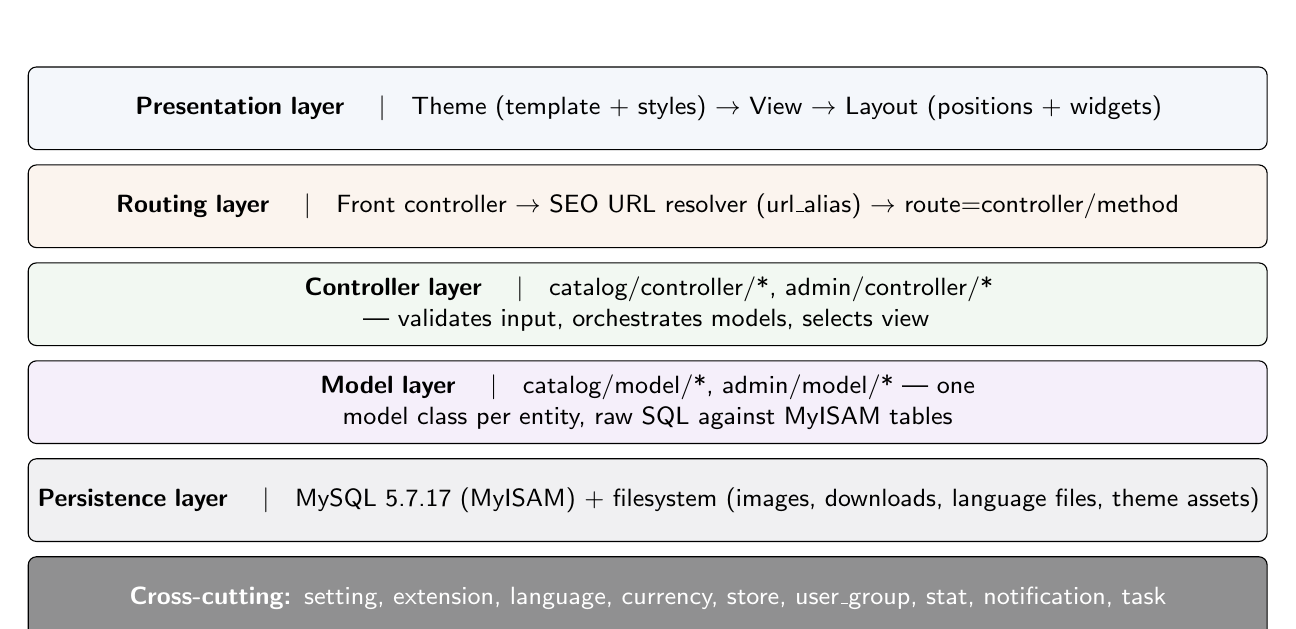
\begin{tikzpicture}[
  layer/.style={draw, rounded corners=3pt, text width=15.5cm,
                minimum height=1.05cm, align=center, font=\small\sffamily},
]
  \node[layer, fill=nodefill]                (presentation) {\textbf{Presentation layer} \quad\textbar\quad Theme (template + styles) $\to$ View $\to$ Layout (positions + widgets)};
  \node[layer, fill=nodefillalt, below=0.18cm of presentation] (routing) {\textbf{Routing layer} \quad\textbar\quad Front controller $\to$ SEO URL resolver (url\_alias) $\to$ route=controller/method};
  \node[layer, fill=nodefillgreen, below=0.18cm of routing] (controller) {\textbf{Controller layer} \quad\textbar\quad catalog/controller/*, admin/controller/* --- validates input, orchestrates models, selects view};
  \node[layer, fill=nodefillpurple, below=0.18cm of controller] (model) {\textbf{Model layer} \quad\textbar\quad catalog/model/*, admin/model/* --- one model class per entity, raw SQL against MyISAM tables};
  \node[layer, fill=nodefillgray, below=0.18cm of model] (persistence) {\textbf{Persistence layer} \quad\textbar\quad MySQL 5.7.17 (MyISAM) + filesystem (images, downloads, language files, theme assets)};
  \node[layer, fill=nodefillgray!60!black, text=white, below=0.18cm of persistence] (crosscutting) {\textbf{Cross-cutting:} setting, extension, language, currency, store, user\_group, stat, notification, task};
\end{tikzpicture}
\caption{Layered view of the Necoyoad architecture. The presentation,
routing, controller, model and persistence layers form the standard
OpenCart-derived MVC pipeline. The bottom band lists cross-cutting
concerns: settings drive configuration everywhere; extensions modify
controller/model behaviour via the event/hook system; language and
currency are loaded once per request; the stat table is written on
every page impression; the notification table is read on every page
load to surface admin/customer alerts; the task scheduler runs out
of band.}
\label{fig:layers}
\end{figure}

\subsection{Four Cross-Cutting Patterns}

The schema exhibits four patterns that recur in domain after domain.
We introduce them here because they are the conceptual key to the
rest of the paper; their concrete realisations are enumerated in
Section~\ref{sec:crosscutting}.

\subsubsection{Pattern 1 --- Polymorphic Object Graph}

A handful of tables are written in a deliberately entity-agnostic way.
The flagship is \texttt{object}, whose columns (\texttt{object\_id},
\texttt{object\_type}, \texttt{parent\_id}, \texttt{parent\_type},
\texttt{status\_id}, \texttt{subtype}, \texttt{status},
\texttt{params}) are explicitly designed to hold \emph{any} kind of
content: a product, a post, a survey, an auction, etc. The
\texttt{object\_type} column is the discriminator. Around
\texttt{object} are four companion tables that follow the same
\texttt{(object\_id, object\_type)} pair as a composite soft
foreign key: \texttt{object\_to\_category},
\texttt{object\_to\_store}, \texttt{description},
\texttt{property}, \texttt{url\_alias}, \texttt{review},
\texttt{stat}, \texttt{notification}. In total there are at least
eleven such polymorphic associations in the schema; they are
enumerated in Appendix~\ref{app:polymorphic}.

\subsubsection{Pattern 2 --- EAV-style Descriptions}

The \texttt{description} table is, in effect, an
Entity-Attribute-Value table specialised for localised rich-text
content. The ``entity'' is the polymorphic \texttt{(object\_id,
object\_type)} pair; the ``value'' is a row containing
\texttt{title}, \texttt{description} (rich HTML), SEO fields
(\texttt{seo\_title}, \texttt{meta\_description},
\texttt{meta\_keywords}) and a free-form \texttt{params} text.
The ``attribute'' dimension is the \texttt{language\_id}. This
single table replaces what would, in vanilla OpenCart, be a dozen
separate \texttt{<entity>\_description} tables.

\subsubsection{Pattern 3 --- Multi-Store Scoping}

The \texttt{store} table lists stores. Each store is identified by
an integer \texttt{store\_id} and has a \texttt{folder} (filesystem
root for that store's assets) and an \texttt{owner\_id}. The
\texttt{customer}, \texttt{menu}, \texttt{notification},
\texttt{product\_attribute}, \texttt{review}, \texttt{search},
\texttt{stat}, \texttt{task}, \texttt{template}, \texttt{theme},
\texttt{widget} tables all carry a \texttt{store\_id} column, and
the polymorphic junction \texttt{object\_to\_store} allows any
content object to be visible in zero, one, many or all stores.
The \texttt{setting} table is also keyed on \texttt{store\_id}, so
each store can have its own configuration overrides. This is a
``multi-tenant within one database'' model.

\subsubsection{Pattern 4 --- Multi-Language Scoping}

The \texttt{language} table is the master list of supported
languages. The \texttt{description}, \texttt{url\_alias},
\texttt{product\_option\_description},
\texttt{product\_option\_value\_description} and
\texttt{product\_tags} tables are all keyed on
\texttt{language\_id}. The \texttt{order} table records the
\texttt{language\_id} at order time so that invoices can be
re-rendered in the customer's original language. The combination
of multi-store and multi-language gives the system a $S \times L$
matrix of presentation surfaces.

\subsection{Status Convention}

A surprisingly important convention is the use of a
\texttt{status} column almost everywhere, with remarkably varied
semantics:

\begin{itemize}[leftmargin=1.6em,itemsep=2pt]
  \item \texttt{int(1)} (0 or 1) on most tables: simple on/off.
  \item \texttt{enum('-1','0','1','')} on \texttt{object}: a 3-state
        ``deleted / disabled / enabled'' lifecycle, with an empty-string
        state for backwards compatibility.
  \item \texttt{varchar(255) DEFAULT '1'} on \texttt{status} (the table):
        a free-form status code that other tables reference via
        \texttt{status\_id}. This is the closest the schema comes to a
        normalised status table.
  \item \texttt{int(5)} on \texttt{order\_history.order\_status\_id}:
        a numeric reference into a status lookup (which in this dump
        is not present as its own table, suggesting it lives in
        \texttt{setting} or in code).
\end{itemize}

The lack of a single, uniform status convention is itself a finding:
different modules grew their own conventions over time.

% ============================================================
\section{Schema Walkthrough by Domain}\label{sec:schema}
% ============================================================

This section is the heart of the document. For each functional domain
we give: a short narrative, an Entity-Relationship Diagram (ERD) drawn
in TikZ, and a table-by-table commentary on the columns that are not
self-explanatory. ERDs use the following conventions: solid boxes are
entity tables; dotted boxes are junction/lookup tables; arrows are
soft foreign keys (MyISAM has no real ones); the
\texttt{(object\_id, object\_type)} polymorphic pair is drawn with a
double-headed arrow.

\subsection{Domain 1 --- The Polymorphic Object Spine}\label{sec:spine}

Before any specific domain, we must lay out the polymorphic spine,
because every other domain hangs off it. The spine consists of six
core tables (\texttt{object}, \texttt{description}, \texttt{property},
\texttt{status}, \texttt{object\_to\_category},
\texttt{object\_to\_store}) and four satellite tables that are
polymorphic by convention (\texttt{url\_alias}, \texttt{review},
\texttt{notification}, \texttt{stat}).

\begin{figure}[htbp]
\centering
\resizebox{\columnwidth}{!}{%
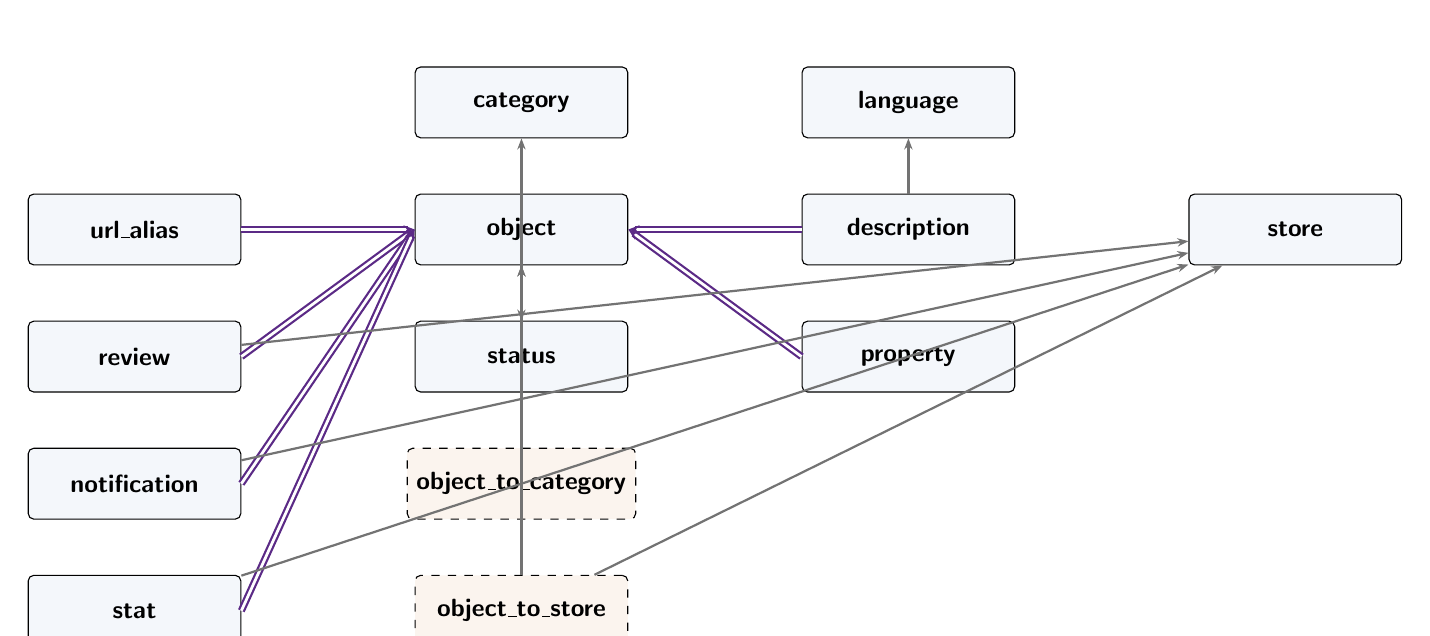
\begin{tikzpicture}[
  entity/.style={draw, rounded corners=2pt, minimum width=2.7cm, minimum height=0.9cm, align=center, font=\small\sffamily, fill=nodefill},
  junction/.style={draw, rounded corners=2pt, minimum width=2.7cm, minimum height=0.9cm, align=center, font=\small\sffamily, fill=nodefillalt, dashed},
  arr/.style={-{Stealth[length=4pt]}, thick, black!55},
  parr/.style={-{Stealth[length=4pt]}, thick, necoyoad-purple, double, double distance=1pt}
]
  \node[entity] (object) {\textbf{object}};
  \node[entity, right=2.2cm of object] (description) {\textbf{description}};
  \node[entity, below=0.7cm of description] (property) {\textbf{property}};
  \node[entity, below=0.7cm of object] (status) {\textbf{status}};
  \node[junction, below=0.7cm of status] (o2c) {\textbf{object\_to\_category}};
  \node[junction, below=0.7cm of o2c] (o2s) {\textbf{object\_to\_store}};

  \node[entity, left=2.2cm of object] (urlalias) {\textbf{url\_alias}};
  \node[entity, below=0.7cm of urlalias] (review) {\textbf{review}};
  \node[entity, below=0.7cm of review] (notif) {\textbf{notification}};
  \node[entity, below=0.7cm of notif] (stat) {\textbf{stat}};

  \node[entity, above=0.7cm of object] (category) {\textbf{category}};
  \node[entity, above=0.7cm of description] (language) {\textbf{language}};
  \node[entity, right=2.2cm of description] (store) {\textbf{store}};

  \draw[parr] (description.west) -- (object.east);
  \draw[parr] (property.west) -- (object.east);
  \draw[parr] (urlalias.east) -- (object.west);
  \draw[parr] (review.east) -- (object.west);
  \draw[parr] (notif.east) -- (object.west);
  \draw[parr] (stat.east) -- (object.west);

  \draw[arr] (object) -- (status);
  \draw[arr] (o2c) -- (object);
  \draw[arr] (o2c) -- (category);
  \draw[arr] (o2s) -- (object);
  \draw[arr] (o2s) -- (store);
  \draw[arr] (description) -- (language);
  \draw[arr] (review) -- (store);
  \draw[arr] (notif) -- (store);
  \draw[arr] (stat) -- (store);
\end{tikzpicture}%
}
\caption{The polymorphic object spine. Six core tables and four
satellite tables all reference the object table via the polymorphic
pair (object\_id, object\_type), shown as a double-headed purple
arrow. The category and store tables are referenced both directly
and indirectly. The status table is the normalised lookup for
state codes.}
\label{fig:spine}
\end{figure}

The \texttt{object} table is the most interesting table in the entire
schema. Its columns explicitly document, via SQL comments, the intent:

\begin{tcolorbox}[enhanced,colback=nodefillgray,colframe=black!40,boxrule=0.3pt,arc=2pt,left=8pt,right=8pt,top=4pt,bottom=4pt,fontupper=\small\ttfamily]
object\_id      INT         -- primary key\\
object\_type    VARCHAR(100) -- 'product', 'post', 'survey', ...\\
parent\_id      INT          -- tree support (categories, subcategories)\\
parent\_type    VARCHAR(100) -- 'product\_category', 'post\_category', ...\\
status\_id      INT          -- FK to status table\\
subtype        VARCHAR(100) -- 'digital', 'normal', 'auction', ...\\
status         ENUM('-1','0','1','')  -- -1:deleted, 0:disabled, 1:enabled\\
params         TEXT         -- 'anything, arrays, classes, objects, strings'\\
sort\_order    INT\\
date\_added    TIMESTAMP DEFAULT CURRENT\_TIMESTAMP\\
date\_modified DATETIME
\end{tcolorbox}

The comment on \texttt{params} --- ``anything, arrays, classes, objects,
strings'' --- is the most candid admission in the entire schema: this
column is a serialised blob of arbitrary PHP data, almost certainly
\texttt{serialize()}/\texttt{unserialize()} or
\texttt{json\_encode()}/\texttt{json\_decode()}. The same pattern
recurs on \texttt{banner.params}, \texttt{customer\_group.params},
\texttt{extension.settings}, \texttt{widget.settings},
\texttt{menu.route}, \texttt{product\_attribute.params} (no, wait ---
\texttt{product\_attribute} has no params; but \texttt{property}
has \texttt{value} which is explicitly \texttt{TEXT} and used for
``anything''). At least seven tables carry a \texttt{params} or
\texttt{settings} \texttt{TEXT} column whose payload is a PHP
serialised value. This is a deliberate escape hatch from the
relational model and is the second cross-cutting pattern (after
polymorphic associations).

\subsection{Domain 2 --- Catalog and Products}\label{sec:catalog}

The catalog domain is the largest functional area, with thirteen tables.
It is also the most OpenCart-flavoured: the table names
(\texttt{product}, \texttt{product\_to\_category},
\texttt{product\_option}, \texttt{product\_option\_value},
\texttt{product\_discount}, \texttt{product\_special},
\texttt{product\_image}, \texttt{product\_related},
\texttt{product\_tags}, \texttt{product\_to\_download},
\texttt{manufacturer}) are essentially identical to OpenCart 1.5/2.x,
with the addition of \texttt{product\_type},
\texttt{product\_attribute}, \texttt{product\_attribute\_group}, and
\texttt{product\_to\_zone}.

\begin{figure}[htbp]
\centering
\resizebox{\columnwidth}{!}{%
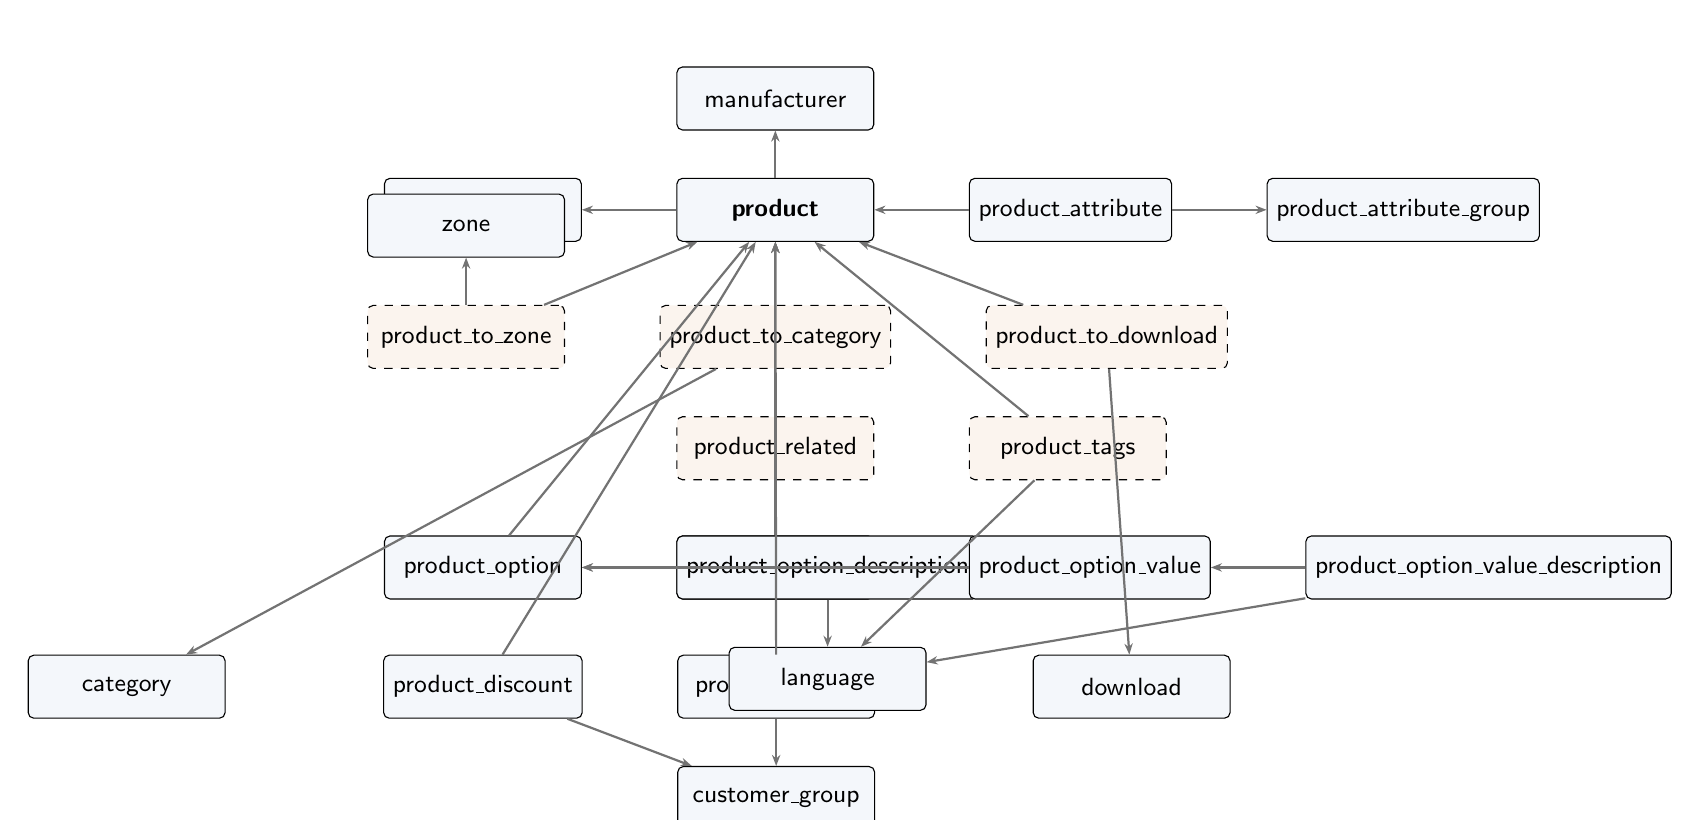
\begin{tikzpicture}[
  entity/.style={draw, rounded corners=2pt, minimum width=2.5cm, minimum height=0.8cm, align=center, font=\small\sffamily, fill=nodefill},
  junction/.style={draw, rounded corners=2pt, minimum width=2.5cm, minimum height=0.8cm, align=center, font=\small\sffamily, fill=nodefillalt, dashed},
  arr/.style={-{Stealth[length=4pt]}, thick, black!55}
]
  \node[entity] (product) {\textbf{product}};
  \node[entity, above=0.6cm of product] (mfr) {manufacturer};
  \node[entity, left=1.2cm of product] (ptype) {product\_type};
  \node[entity, right=1.2cm of product] (pattr) {product\_attribute};
  \node[entity, right=1.2cm of pattr] (pagrp) {product\_attribute\_group};

  \node[junction, below=0.8cm of product] (p2c) {product\_to\_category};
  \node[junction, right=1.2cm of p2c] (p2d) {product\_to\_download};
  \node[junction, left=1.2cm of p2c] (p2z) {product\_to\_zone};
  \node[junction, below=0.6cm of p2c] (p2rel) {product\_related};
  \node[junction, right=1.2cm of p2rel] (ptags) {product\_tags};

  \node[entity, below=0.7cm of p2rel] (pimg) {product\_image};
  \node[entity, left=1.2cm of pimg] (popt) {product\_option};
  \node[entity, right=1.2cm of popt] (poptdesc) {product\_option\_description};
  \node[entity, right=1.2cm of pimg] (pov) {product\_option\_value};
  \node[entity, right=1.2cm of pov] (povdesc) {product\_option\_value\_description};

  \node[entity, below=0.7cm of popt] (pdisc) {product\_discount};
  \node[entity, right=1.2cm of pdisc] (pspec) {product\_special};

  \node[entity, left=2.0cm of pdisc] (cat) {category};
  \node[entity, right=2.0cm of pspec] (download) {download};
  \node[entity, below=0.6cm of pspec] (cgroup) {customer\_group};
  \node[entity, below=0.6cm of poptdesc] (lang) {language};
  \node[entity, above=0.6cm of p2z] (zone) {zone};

  \draw[arr] (product) -- (mfr);
  \draw[arr] (product) -- (ptype);
  \draw[arr] (pattr) -- (pagrp);
  \draw[arr] (pattr) -- (product);
  \draw[arr] (p2c) -- (product);
  \draw[arr] (p2c) -- (cat);
  \draw[arr] (p2d) -- (product);
  \draw[arr] (p2d) -- (download);
  \draw[arr] (p2z) -- (zone);
  \draw[arr] (p2z) -- (product);
  \draw[arr] (p2rel) -- (product);
  \draw[arr] (ptags) -- (product);
  \draw[arr] (ptags) -- (lang);
  \draw[arr] (pimg) -- (product);
  \draw[arr] (popt) -- (product);
  \draw[arr] (poptdesc) -- (popt);
  \draw[arr] (poptdesc) -- (lang);
  \draw[arr] (pov) -- (popt);
  \draw[arr] (povdesc) -- (pov);
  \draw[arr] (povdesc) -- (lang);
  \draw[arr] (pdisc) -- (product);
  \draw[arr] (pdisc) -- (cgroup);
  \draw[arr] (pspec) -- (product);
  \draw[arr] (pspec) -- (cgroup);
\end{tikzpicture}%
}
\caption{Catalog domain ERD. The product table is the hub. Thirteen
satellite tables cover taxonomies, localisation, inventory-by-zone,
media, merchandising and extensibility. See the body text for the
full per-table breakdown.}
\label{fig:catalog}
\end{figure}

\subsubsection{Notable Columns in \texttt{product}}

\begin{itemize}[leftmargin=1.6em,itemsep=2pt]
  \item \texttt{owner\_id} --- the customer or admin who owns the product.
        This is non-OpenCart and suggests a vendor/marketplace model where
        customers can be sellers.
  \item \texttt{product\_type} \texttt{VARCHAR(255)} --- a free-form type
        discriminator (digital, normal, auction, ...). It is also backed
        by the \texttt{product\_type} lookup table; the relationship
        between the two is not enforced.
  \item \texttt{sku}, \texttt{model} (unique), \texttt{location} ---
        standard inventory identifiers.
  \item \texttt{quantity}, \texttt{subtract}, \texttt{minimum},
        \texttt{stock\_status\_id} --- standard OpenCart stock controls.
  \item \texttt{price} (gross) and \texttt{cost} --- both stored, so the
        system can compute margin in reports.
  \item \texttt{weight}, \texttt{length}, \texttt{width}, \texttt{height}
        plus their class IDs --- physical dimensions for shipping.
  \item \texttt{date\_available} --- the date from which the product is
        listed. Combined with \texttt{status}, this gives a
        time-windowed visibility model.
  \item \texttt{viewed} --- a denormalised view counter, incremented
        per product page load.
  \item \texttt{sort\_order} --- manual ordering.
\end{itemize}

\subsubsection{The Three Pricing Tiers}

The catalog has three distinct pricing mechanisms that layer on top of
the base \texttt{product.price}:

\begin{enumerate}[leftmargin=1.6em,itemsep=2pt]
  \item \textbf{\texttt{product\_discount}} --- quantity breaks scoped
        to a \texttt{customer\_group\_id} and a date window
        (\texttt{date\_start}, \texttt{date\_end}). Standard OpenCart.
  \item \textbf{\texttt{product\_special}} --- a promotional price,
        also scoped to a \texttt{customer\_group\_id} and a date
        window. Standard OpenCart.
  \item \textbf{\texttt{coupon}} (see Section~\ref{sec:orders}) ---
        a checkout-time discount applied via a code.
\end{enumerate}

The resolution order at display time is, by OpenCart convention:
\texttt{special} (if active) $\to$ \texttt{discount} (if quantity threshold
met) $\to$ base \texttt{price}. The application is responsible for this
resolution; the database stores all three independently.

\subsubsection{Product Attributes vs.\ Product Options}

The schema distinguishes two easily-confused concepts:

\begin{itemize}[leftmargin=1.6em,itemsep=2pt]
  \item \textbf{Product attributes} (\texttt{product\_attribute} +
        \texttt{product\_attribute\_group}) are \emph{display-only}
        specifications: e.g.\ ``Screen size: 5.5\,in'', ``Battery:
        3000\,mAh''. They are defined per-store (there is a
        \texttt{store\_id} column), grouped, typed
        (\texttt{type}, \texttt{pattern}, \texttt{default},
        \texttt{required}) and are not directly orderable. The
        \texttt{group}, \texttt{label}, \texttt{name} columns imply
        a form-builder UI.
  \item \textbf{Product options} (\texttt{product\_option} +
        \texttt{product\_option\_description} +
        \texttt{product\_option\_value} +
        \texttt{product\_option\_value\_description}) are
        \emph{orderable} variants: e.g.\ ``Colour: Red / Blue'',
        ``Size: S / M / L''. Each value has its own
        \texttt{quantity}, \texttt{subtract} flag, \texttt{price}
        delta and \texttt{prefix} (\texttt{+} or \texttt{-}). They
        are language-translated via the two
        \texttt{\_description} tables.
\end{itemize}

\subsubsection{Tags and Taxonomy}

\texttt{product\_tags} (note the plural --- OpenCart convention) is a
separate, language-keyed tag table. The primary key is the composite
\texttt{(product\_id, tag, language\_id)}, which prevents duplicate
tags per language but allows the same tag in different languages.
The \texttt{product\_to\_category} junction is the primary taxonomy;
\texttt{product\_to\_zone} restricts a product's availability to
certain zones (likely for shipping or regulatory reasons); and
\texttt{product\_related} is a self-referential many-to-many
``related products'' table.

\subsection{Domain 3 --- Customers, Addresses and Reviews}\label{sec:customers}

\begin{figure}[htbp]
\centering
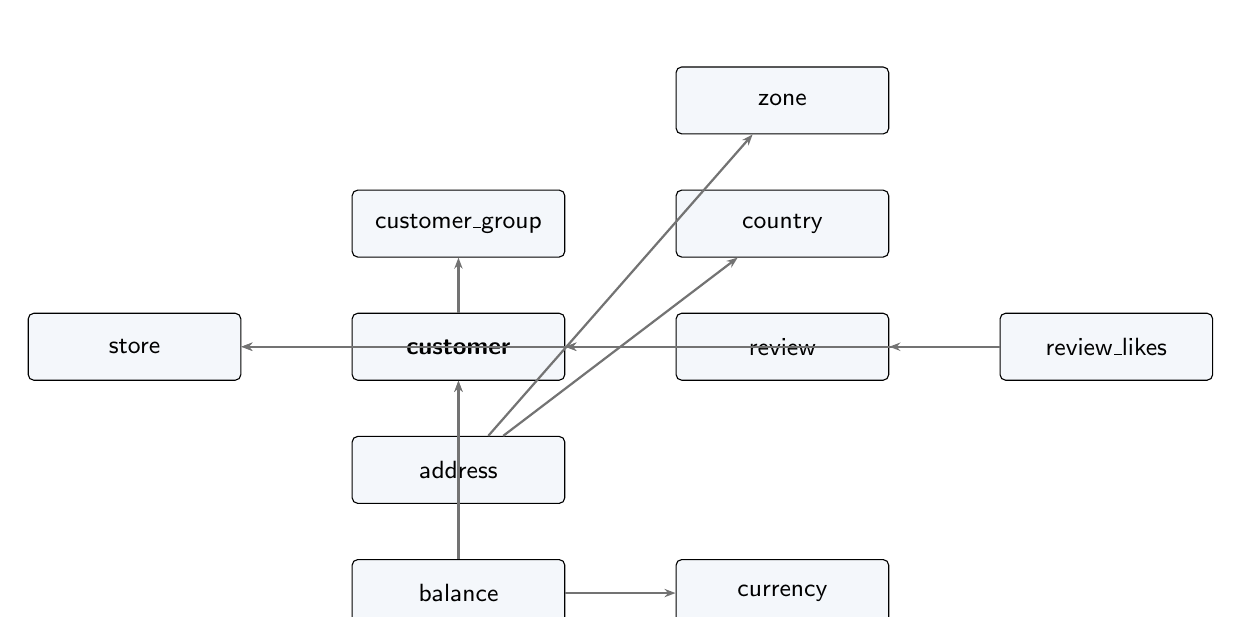
\begin{tikzpicture}[
  entity/.style={draw, rounded corners=2pt, minimum width=2.7cm, minimum height=0.85cm, align=center, font=\small\sffamily, fill=nodefill},
  junction/.style={draw, rounded corners=2pt, minimum width=2.7cm, minimum height=0.85cm, align=center, font=\small\sffamily, fill=nodefillalt, dashed},
  arr/.style={-{Stealth[length=4pt]}, thick, black!55}
]
  \node[entity] (customer) {\textbf{customer}};
  \node[entity, above=0.7cm of customer] (cgroup) {customer\_group};
  \node[entity, left=1.4cm of customer] (store) {store};
  \node[entity, below=0.7cm of customer] (address) {address};
  \node[entity, below=0.7cm of address] (balance) {balance};
  \node[entity, right=1.4cm of customer] (review) {review};
  \node[entity, right=1.4cm of review] (rlikes) {review\_likes};
  \node[entity, above=0.7cm of review] (country) {country};
  \node[entity, above=0.7cm of country] (zone) {zone};
  \node[entity, right=1.4cm of balance] (currency) {currency};

  \draw[arr] (customer) -- (cgroup);
  \draw[arr] (customer) -- (store);
  \draw[arr] (address) -- (customer);
  \draw[arr] (address) -- (country);
  \draw[arr] (address) -- (zone);
  \draw[arr] (balance) -- (customer);
  \draw[arr] (balance) -- (currency);
  \draw[arr] (review) -- (customer);
  \draw[arr] (review) -- (store);
  \draw[arr] (rlikes) -- (review);
  \draw[arr] (rlikes) -- (customer);
\end{tikzpicture}
\caption{Customer domain ERD. A customer belongs to one customer\_group
(drives pricing and permissions), is registered against a store, and
has one or more addresses. The balance table is a per-currency
wallet ledger; review and review\_likes form a small social layer.}
\label{fig:customers}
\end{figure}

\subsubsection{Notable Columns in \texttt{customer}}

The \texttt{customer} table is significantly extended beyond vanilla
OpenCart. The Venezuelan context is visible in several places:

\begin{itemize}[leftmargin=1.6em,itemsep=2pt]
  \item \texttt{rif} \texttt{VARCHAR(12)} --- the Venezuelan
        \emph{Registro de Informaci\'on Fiscal} tax identifier,
        used for both individuals and companies. This is a
        strong signal that the application was built for the
        Venezuelan market.
  \item \texttt{company} \texttt{VARCHAR(90)} --- the customer's
        company name (relevant because the RIF can be corporate).
  \item \texttt{activation\_code} \texttt{VARCHAR(255)} --- the
        account-activation token sent by email at signup.
  \item \texttt{photo} \texttt{VARCHAR(255)} --- a filesystem
        path to the customer's avatar.
  \item \texttt{birthday}, \texttt{congrats} --- birthday and a
        flag for whether the customer has been sent birthday
        greetings (likely via the campaign system).
  \item \texttt{referenced\_by} --- a customer-referral field.
  \item \texttt{cart} \texttt{TEXT} --- a serialised PHP array
        of the customer's shopping cart, persisted between
        sessions. This is the OpenCart convention.
  \item \texttt{banned}, \texttt{approved}, \texttt{complete},
        \texttt{visits}, \texttt{ip} --- moderation and audit
        fields.
  \item \texttt{sex} \texttt{CHAR(1)} --- gender.
  \item \texttt{password} \texttt{VARCHAR(100)} --- the password
        hash (the length suggests bcrypt or Argon2; the legacy
        OpenCart md5+salt would fit in 40 characters).
\end{itemize}

\subsubsection{The Wallet: \texttt{balance}}

The \texttt{balance} table is a per-customer, per-currency ledger.
Each row records: a \texttt{type} (3-char code, likely \texttt{cr}
for credit and \texttt{db} for debit), an \texttt{amount}, a
\texttt{description}, three running totals
(\texttt{amount\_available}, \texttt{amount\_blocked},
\texttt{amount\_total}) and a currency snapshot
(\texttt{currency\_code}, \texttt{currency\_value},
\texttt{currency\_title}). The presence of a ``blocked'' amount
suggests the wallet can have funds reserved (e.g.\ for a pending
order) and released (when the order completes) or voided (when the
order is cancelled). This is the mechanism that ties the wallet to
the order-payment flow (Section~\ref{sec:payments}).

\subsubsection{Reviews and Likes}

The \texttt{review} table is polymorphic: it can attach to any
\texttt{object\_id}/\texttt{object\_type} pair (a product, a post,
etc.). It has a \texttt{parent\_id} for threaded replies, an
\texttt{author} string (so non-customers can also review), a
\texttt{rating} (1--5), and the standard status / date fields.
The \texttt{review\_likes} table records per-customer
\texttt{like}/\texttt{dislike} votes on reviews, with a unique key
on \texttt{(review\_id, customer\_id)} to prevent double-voting.

\subsection{Domain 4 --- Orders, Coupons and Checkout}\label{sec:orders}

\begin{figure}[htbp]
\centering
\resizebox{\columnwidth}{!}{%
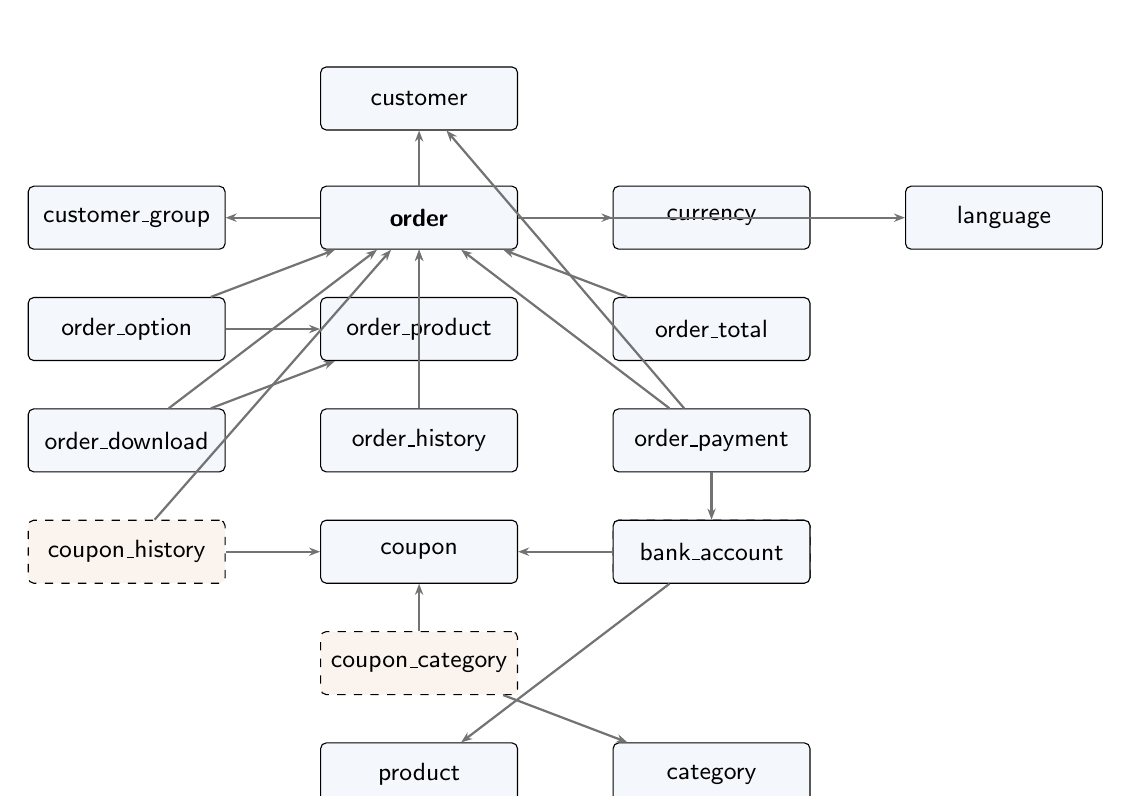
\begin{tikzpicture}[
  entity/.style={draw, rounded corners=2pt, minimum width=2.5cm, minimum height=0.8cm, align=center, font=\small\sffamily, fill=nodefill},
  junction/.style={draw, rounded corners=2pt, minimum width=2.5cm, minimum height=0.8cm, align=center, font=\small\sffamily, fill=nodefillalt, dashed},
  arr/.style={-{Stealth[length=4pt]}, thick, black!55}
]
  \node[entity] (order) {\textbf{order}};
  \node[entity, above=0.7cm of order] (customer) {customer};
  \node[entity, left=1.2cm of order] (cgroup) {customer\_group};
  \node[entity, right=1.2cm of order] (currency) {currency};
  \node[entity, right=1.2cm of currency] (lang) {language};
  \node[entity, below=0.6cm of order] (oprod) {order\_product};
  \node[entity, left=1.2cm of oprod] (ooption) {order\_option};
  \node[entity, right=1.2cm of oprod] (ototal) {order\_total};
  \node[entity, below=0.6cm of oprod] (ohist) {order\_history};
  \node[entity, left=1.2cm of ohist] (odl) {order\_download};
  \node[entity, right=1.2cm of ohist] (opay) {order\_payment};
  \node[entity, below=0.6cm of ohist] (coupon) {coupon};
  \node[junction, left=1.2cm of coupon] (cph) {coupon\_history};
  \node[junction, right=1.2cm of coupon] (cpp) {coupon\_product};
  \node[junction, below=0.6cm of coupon] (cpc) {coupon\_category};
  \node[entity, below=0.6cm of opay] (bankacc) {bank\_account};
  \node[entity, below=0.6cm of cpc] (product) {product};
  \node[entity, right=1.2cm of product] (category) {category};

  \draw[arr] (order) -- (customer);
  \draw[arr] (order) -- (cgroup);
  \draw[arr] (order) -- (currency);
  \draw[arr] (order) -- (lang);
  \draw[arr] (oprod) -- (order);
  \draw[arr] (ooption) -- (order);
  \draw[arr] (ooption) -- (oprod);
  \draw[arr] (ototal) -- (order);
  \draw[arr] (ohist) -- (order);
  \draw[arr] (odl) -- (order);
  \draw[arr] (odl) -- (oprod);
  \draw[arr] (opay) -- (order);
  \draw[arr] (opay) -- (customer);
  \draw[arr] (opay) -- (bankacc);
  \draw[arr] (cph) -- (coupon);
  \draw[arr] (cph) -- (order);
  \draw[arr] (cpp) -- (coupon);
  \draw[arr] (cpp) -- (product);
  \draw[arr] (cpc) -- (coupon);
  \draw[arr] (cpc) -- (category);
\end{tikzpicture}%
}
\caption{Order and coupon ERD. The order table is the hub. It
snapshots the customer, address, shipping and payment details at
order time. Each order\_product line carries its options (via
order\_option) and any associated downloads (via order\_download).
The order\_total table holds the ordered list of total-line
computations. The order\_payment table records manual bank-transfer
payments. Coupons are scoped to products and categories, and have a
usage history.}
\label{fig:orders}
\end{figure}

\subsubsection{The Snapshot Pattern in \texttt{order}}

The \texttt{order} table is a textbook example of the \emph{snapshot}
pattern: rather than normalising the customer's name, address, phone,
email, shipping address and payment address into references to the
\texttt{customer} and \texttt{address} tables, the order copies all of
these fields verbatim into its own columns
(\texttt{firstname}, \texttt{lastname}, \texttt{telephone}, \texttt{rif},
\texttt{email}, \texttt{shipping\_firstname}, \texttt{shipping\_lastname},
\ldots, \texttt{payment\_firstname}, \texttt{payment\_lastname}, \ldots).
This is standard practice in commerce systems: an order is a legal
artifact and must remain readable even if the customer later changes
their name or deletes their account. The trade-off is a wide, denormalised
table; the \texttt{order} table has 43 columns.

\subsubsection{Order Status and History}

The \texttt{order} table has a single \texttt{order\_status\_id}
column (current status). The full status history is kept in
\texttt{order\_history}, where each row records an
\texttt{order\_status\_id} change, a \texttt{notify} flag (whether
the customer was emailed about this transition), a \texttt{comment}
and a timestamp. This is a standard OpenCart state-log pattern.

\subsubsection{\texttt{order\_total} --- The Extension Point}

The \texttt{order\_total} table is the database side of one of
OpenCart's most important extension points. Each row is a single
line in the cart total: \texttt{title} (e.g.\ ``Sub-Total''),
\texttt{text} (the formatted, localised amount, e.g.\ ``USD\,120.00''),
\texttt{value} (the numeric amount), \texttt{sort\_order}. The
application computes these lines by iterating over a set of
``total extension'' classes (sub-total, shipping, tax, coupon,
voucher, reward points, ...) installed via the
\texttt{extension} table. Each extension contributes one or more
rows to \texttt{order\_total} when the order is finalised. The
\texttt{order.total} column is the sum of all
\texttt{order\_total.value} rows for that order.

\subsubsection{\texttt{order\_payment} --- Manual Bank Transfers}

The \texttt{order\_payment} table records manual payment
notifications: the customer reports that they have made a bank
transfer (transaction number, date, originating bank, amount,
comment), and an admin later marks the row as confirmed by
setting its \texttt{order\_payment\_status\_id}. Each row links
to a \texttt{bank\_account} (the merchant's account that
received the transfer). This is the typical flow in
Venezuelan e-commerce, where credit-card payment gateways
were unreliable for years and bank transfers became the default.

\subsubsection{Coupons}

The \texttt{coupon} table is the OpenCart standard: a code, a
discount \texttt{type} (\texttt{P} percentage or \texttt{F} fixed),
a \texttt{discount} amount, a \texttt{total} minimum cart total,
a date window, \texttt{uses\_total} (max global uses),
\texttt{uses\_customer} (max uses per customer, stored as
\texttt{VARCHAR(11)} --- possibly ``'' or ``N''), a
\texttt{logged} flag (must the customer be logged in?) and a
\texttt{shipping} flag (does the coupon free shipping?).
The \texttt{coupon\_product} and \texttt{coupon\_category}
junctions scope the coupon to specific products or categories.
The \texttt{coupon\_history} table logs every use.

\subsection{Domain 5 --- Banking and Wallet}\label{sec:payments}

\begin{figure}[htbp]
\centering
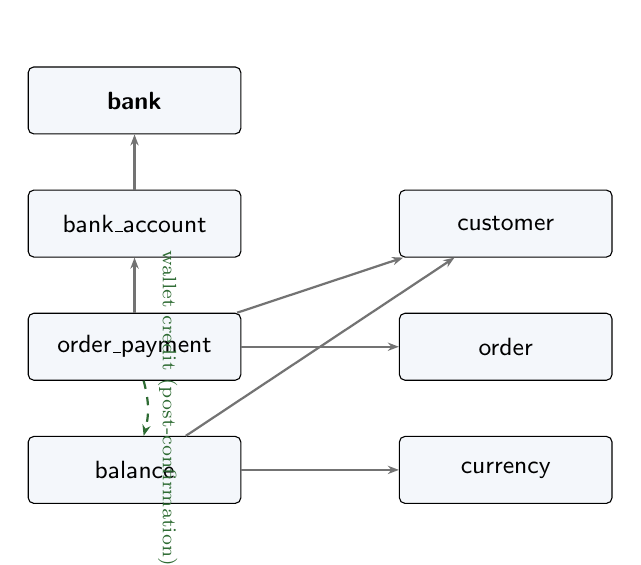
\begin{tikzpicture}[
  entity/.style={draw, rounded corners=2pt, minimum width=2.7cm, minimum height=0.85cm, align=center, font=\small\sffamily, fill=nodefill},
  arr/.style={-{Stealth[length=4pt]}, thick, black!55}
]
  \node[entity] (bank) {\textbf{bank}};
  \node[entity, below=0.7cm of bank] (bacc) {bank\_account};
  \node[entity, below=0.7cm of bacc] (opay) {order\_payment};
  \node[entity, right=2.0cm of opay] (order) {order};
  \node[entity, above=0.7cm of order] (customer) {customer};
  \node[entity, below=0.7cm of opay] (balance) {balance};
  \node[entity, right=2.0cm of balance] (currency) {currency};

  \draw[arr] (bacc) -- (bank);
  \draw[arr] (opay) -- (bacc);
  \draw[arr] (opay) -- (order);
  \draw[arr] (opay) -- (customer);
  \draw[arr] (balance) -- (customer);
  \draw[arr] (balance) -- (currency);
  \draw[arr, dashed, necoyoad-green] (opay) edge[bend left=15] node[font=\scriptsize, above, sloped] {wallet credit (post-confirmation)} (balance);
\end{tikzpicture}
\caption{Banking and wallet domain. The merchant maintains a
directory of banks (\texttt{bank}) and their accounts
(\texttt{bank\_account}). The customer reports a transfer via
\texttt{order\_payment}; after admin confirmation, the wallet
\texttt{balance} for that customer is credited (dashed green arrow
--- inferred post-confirmation side-effect, not enforced by the
database).}
\label{fig:banking}
\end{figure}

The banking domain is small but operationally important. The
\texttt{bank} table holds the master list of banks (name, logo
image, dates). The \texttt{bank\_account} table records each
merchant account: the owning \texttt{bank\_id}, the account
\texttt{number} (unique), the \texttt{accountholder} name, the
\texttt{type} (savings, checking, ...), the contact \texttt{email},
the \texttt{rif} (the merchant's tax ID for that account), and a
\texttt{status}. The \texttt{order\_payment} table, described in
Section~\ref{sec:orders}, references \texttt{bank\_account}.

The dashed arrow in Figure~\ref{fig:banking} is an inferred
side-effect: when an admin confirms an \texttt{order\_payment}
(by advancing its \texttt{order\_payment\_status\_id}), the
application is expected to also write a corresponding credit row
to the customer's \texttt{balance} ledger. The database does not
enforce this; it is an application-level invariant.

\subsection{Domain 6 --- CMS, Posts, Banners, Menus}\label{sec:cms}

\begin{figure}[htbp]
\centering
\resizebox{\columnwidth}{!}{%
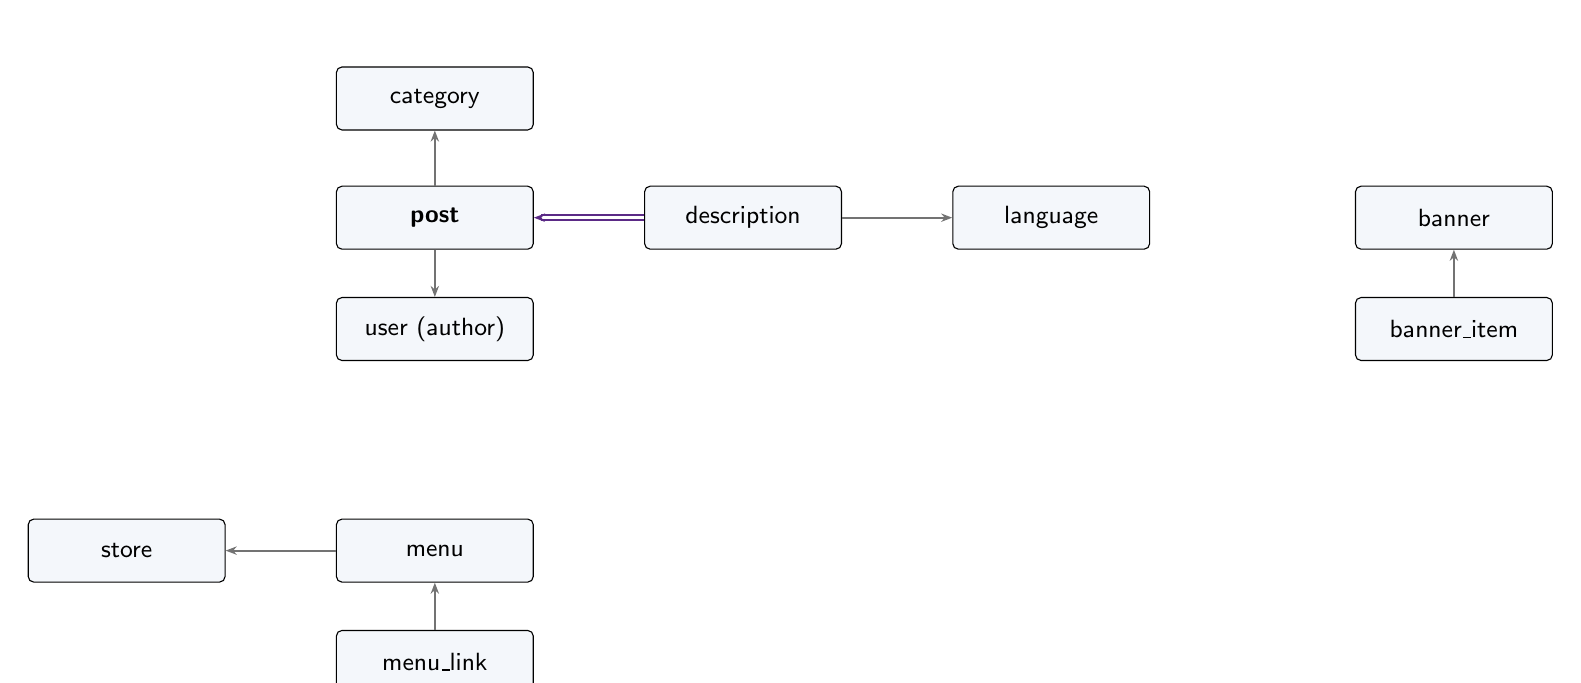
\begin{tikzpicture}[
  entity/.style={draw, rounded corners=2pt, minimum width=2.5cm, minimum height=0.8cm, align=center, font=\small\sffamily, fill=nodefill},
  junction/.style={draw, rounded corners=2pt, minimum width=2.5cm, minimum height=0.8cm, align=center, font=\small\sffamily, fill=nodefillalt, dashed},
  arr/.style={-{Stealth[length=4pt]}, thick, black!55},
  parr/.style={-{Stealth[length=4pt]}, thick, necoyoad-purple, double, double distance=1pt}
]
  \node[entity] (post) {\textbf{post}};
  \node[entity, above=0.7cm of post] (cat) {category};
  \node[entity, right=1.4cm of post] (desc) {description};
  \node[entity, right=1.4cm of desc] (lang) {language};
  \node[entity, below=0.6cm of post] (user) {user (author)};

  \node[entity, right=2.6cm of lang] (banner) {banner};
  \node[entity, below=0.6cm of banner] (bitem) {banner\_item};

  \node[entity, below=2.0cm of user] (menu) {menu};
  \node[entity, below=0.6cm of menu] (mlink) {menu\_link};
  \node[entity, left=1.4cm of menu] (store) {store};

  \draw[parr] (desc) -- (post);
  \draw[arr] (desc) -- (lang);
  \draw[arr] (post) -- (user);
  \draw[arr] (post) -- (cat);
  \draw[arr] (bitem) -- (banner);
  \draw[arr] (menu) -- (store);
  \draw[arr] (mlink) -- (menu);
\end{tikzpicture}%
}
\caption{CMS domain. A \texttt{post} is a content node (blog article,
page, custom post type) authored by an admin \texttt{user} and
classified by a polymorphic \texttt{category}. Its localised
title/body/SEO fields live in the \texttt{description} table
(polymorphic, keyed on \texttt{object\_id = post\_id},
\texttt{object\_type = 'post'}), one row per language. Banners and
menu structures are independent subsystems.}
\label{fig:cms}
\end{figure}

\subsubsection{Posts}

The \texttt{post} table is a small but flexible CMS engine.
Each post has: a \texttt{parent\_id} (for hierarchical post
types, e.g.\ a page tree), an \texttt{author\_id} (admin
\texttt{user}), a \texttt{post\_type} discriminator (e.g.\
\texttt{post}, \texttt{page}, \texttt{article}), an image, a
publishing window (\texttt{date\_publish\_start},
\texttt{date\_publish\_end}, \texttt{publish} flag), an
\texttt{allow\_reviews} flag, and a \texttt{template} column
that selects which view template renders the post. The
combination of \texttt{post\_type} + \texttt{template} gives
the system a custom-post-type mechanism reminiscent of
WordPress.

\subsubsection{Banners}

The \texttt{banner} table is interesting because of its
\texttt{jquery\_plugin} and \texttt{params} columns. Each
banner can specify a jQuery slideshow plugin (e.g.\ ``nivo-
slider'', ``bxslider'') and a serialised parameter set.
This is a deliberate extension point: the front-end renders
the banner by loading the named jQuery plugin and feeding it
the banner items and the params. Each \texttt{banner\_item}
is a single slide (image + link + sort order + status).

\subsubsection{Menus}

The \texttt{menu} table stores named menus scoped to a store
(\texttt{store\_id}), with a \texttt{position} (e.g.\
``header'', ``footer'', ``sidebar''), a \texttt{route}
(the page the menu links to by default), a \texttt{default}
flag and a \texttt{status}. The \texttt{menu\_link} table
stores the individual menu items, with a \texttt{parent\_id}
for tree-structured menus, a \texttt{link}, a \texttt{tag}
(the visible label) and a \texttt{sort\_order}.

\subsection{Domain 7 --- Themes, Templates and Widgets}\label{sec:themes}

The presentation layer is a four-table stack that gives the
system a complete visual-customisation surface:
\texttt{template} (the design package),
\texttt{theme} (an instance of a template, scoped to a store
and a user), \texttt{theme\_style} (CSS-rule-level overrides
for a theme), and \texttt{widget} (positioned, configurable
content blocks). A fifth table, \texttt{widget\_landing\_page},
binds a widget to a specific landing page and object type.

\begin{figure}[htbp]
\centering
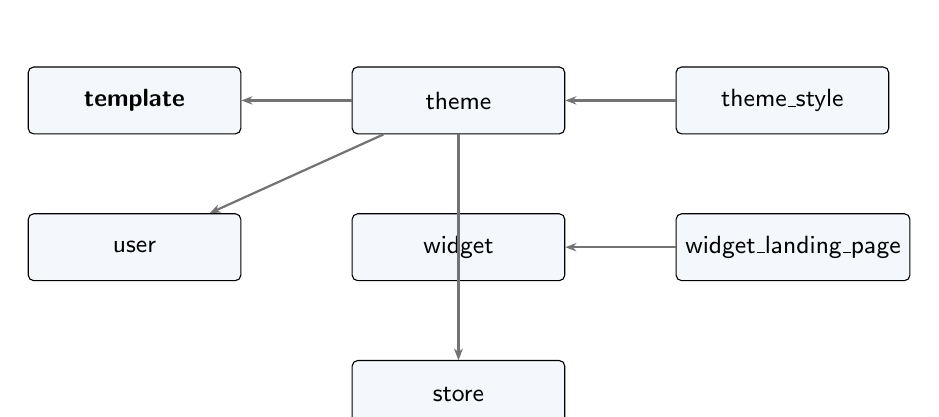
\begin{tikzpicture}[
  entity/.style={draw, rounded corners=2pt, minimum width=2.7cm, minimum height=0.85cm, align=center, font=\small\sffamily, fill=nodefill},
  arr/.style={-{Stealth[length=4pt]}, thick, black!55}
]
  \node[entity] (template) {\textbf{template}};
  \node[entity, right=1.4cm of template] (theme) {theme};
  \node[entity, right=1.4cm of theme] (tstyle) {theme\_style};
  \node[entity, below=1.0cm of theme] (widget) {widget};
  \node[entity, right=1.4cm of widget] (wlp) {widget\_landing\_page};
  \node[entity, below=1.0cm of widget] (store) {store};
  \node[entity, below=1.0cm of template] (user) {user};

  \draw[arr] (theme) -- (template);
  \draw[arr] (tstyle) -- (theme);
  \draw[arr] (theme) -- (store);
  \draw[arr] (theme) -- (user);
  \draw[arr] (widget) -- (store);
  \draw[arr] (wlp) -- (widget);
\end{tikzpicture}
\caption{Presentation stack. A \texttt{template} is a design package
(with versioning and a ``for\_nt\_version'' compatibility field).
A \texttt{theme} is an instantiation of a template for a particular
store and editor (\texttt{user\_id}), with a default flag and a
publishing window. A \texttt{theme\_style} row is a single CSS
rule override (selector, property, value) for a theme. A
\texttt{widget} is a positioned, configurable content block; the
\texttt{widget\_landing\_page} table restricts a widget to a
particular landing page and object type.}
\label{fig:themes}
\end{figure}

\subsubsection{The Template Versioning Column}

The \texttt{template} table has a \texttt{for\_nt\_version}
column. ``nt'' almost certainly stands for ``Necoyoad
Template'' or ``Necoyoad Theme''. The presence of this
column tells us that the platform has its own version
numbering, separate from OpenCart's, and that templates
declare which platform version they target. This is
consistent with the system being a fork or derivative
rather than a vanilla OpenCart install.

\subsubsection{Widgets}

The \texttt{widget} table is one of the most application-
rich tables in the schema. Each widget has:
\texttt{code} (a unique identifier), \texttt{name},
\texttt{extension} (which extension provides this widget's
controller), \texttt{position} (where on the page it
appears), \texttt{app} (which app: ``catalog'',
``admin''), \texttt{order} (sorting), \texttt{settings}
(a serialised PHP blob of widget configuration), and
\texttt{status}. The combination of \texttt{extension}
and \texttt{settings} makes widgets the primary
extension surface for the front-end: an admin can drop a
widget into a position, configure it, and the front
controller dispatches to the widget's controller to
render it.

\subsection{Domain 8 --- Marketing and Campaigns}\label{sec:marketing}

The marketing domain is the most sophisticated subsystem in
the schema after the catalog. It implements a complete
email-marketing pipeline: newsletters, campaigns, contact
lists, per-recipient tracking, link click tracking, and a
queue-based sending engine that runs on the task scheduler.

\begin{figure}[htbp]
\centering
\resizebox{\columnwidth}{!}{%
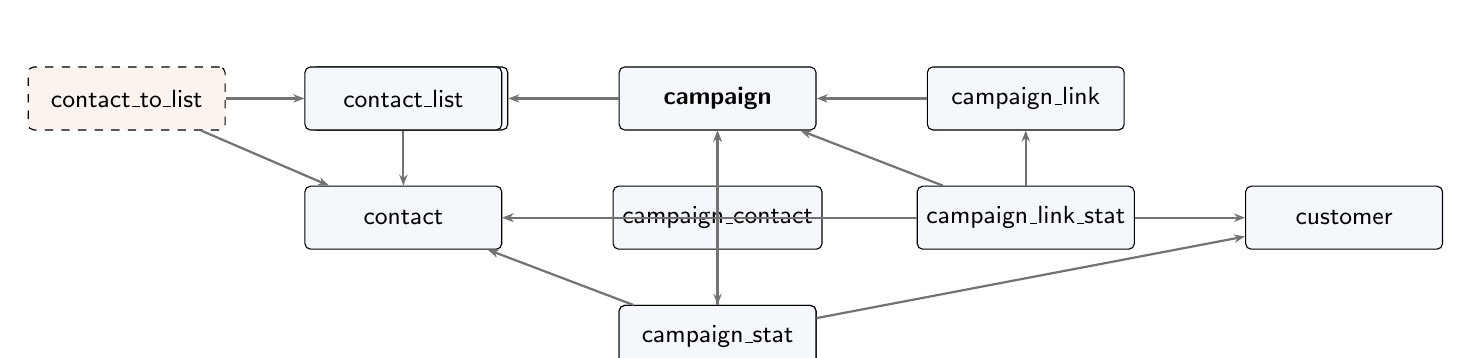
\begin{tikzpicture}[
  entity/.style={draw, rounded corners=2pt, minimum width=2.5cm, minimum height=0.8cm, align=center, font=\small\sffamily, fill=nodefill},
  junction/.style={draw, rounded corners=2pt, minimum width=2.5cm, minimum height=0.8cm, align=center, font=\small\sffamily, fill=nodefillalt, dashed},
  arr/.style={-{Stealth[length=4pt]}, thick, black!55}
]
  \node[entity] (news) {\textbf{newsletter}};
  \node[entity, right=1.4cm of news] (camp) {\textbf{campaign}};
  \node[entity, below=0.7cm of camp] (cc) {campaign\_contact};
  \node[entity, left=1.4cm of cc] (contact) {contact};
  \node[entity, above=0.7cm of contact] (clist) {contact\_list};
  \node[junction, left=1.0cm of clist] (c2l) {contact\_to\_list};
  \node[entity, below=0.7cm of cc] (tq) {task\_queue};
  \node[entity, right=1.4cm of camp] (clink) {campaign\_link};
  \node[entity, below=0.7cm of clink] (cls) {campaign\_link\_stat};
  \node[entity, below=0.7cm of cc] (cs) {campaign\_stat};
  \node[entity, right=1.4cm of cls] (cust) {customer};

  \draw[arr] (camp) -- (news);
  \draw[arr] (cc) -- (camp);
  \draw[arr] (cc) -- (contact);
  \draw[arr] (cc) -- (tq);
  \draw[arr] (c2l) -- (clist);
  \draw[arr] (c2l) -- (contact);
  \draw[arr] (clist) -- (contact);
  \draw[arr] (clink) -- (camp);
  \draw[arr] (cls) -- (clink);
  \draw[arr] (cls) -- (camp);
  \draw[arr] (cls) -- (cust);
  \draw[arr] (cls) -- (contact);
  \draw[arr] (cs) -- (camp);
  \draw[arr] (cs) -- (cust);
  \draw[arr] (cs) -- (contact);
\end{tikzpicture}%
}
\caption{Marketing/CRM domain. A \texttt{newsletter} is a reusable
email body (text + HTML). A \texttt{campaign} is a sending of a
newsletter to a set of contacts. Each
\texttt{campaign\_contact} row is one recipient of one campaign,
linked to a \texttt{task\_queue} entry that drives the actual send.
\texttt{campaign\_link} stores the rewritten, trackable links
inside the email. \texttt{campaign\_stat} records email opens
(per recipient, with full HTTP context). \texttt{campaign\_link\_stat}
records link clicks (per recipient, per link). Contacts are
organised into \texttt{contact\_list}s via the
\texttt{contact\_to\_list} junction.}
\label{fig:marketing}
\end{figure}

\subsubsection{The Campaign Lifecycle}

A campaign has a \texttt{date\_start}, a \texttt{date\_end}, a
\texttt{repeat} field (likely ``once'', ``daily'', ``weekly'',
``monthly''), and several tracking flags:
\texttt{trace\_email} (track opens), \texttt{trace\_click}
(track clicks), \texttt{embed\_image} (embed images vs.\ link
them). The inferred lifecycle is:

\begin{enumerate}[leftmargin=1.6em,itemsep=2pt]
  \item Admin composes a \texttt{newsletter} (text + HTML body).
  \item Admin creates a \texttt{campaign} that uses the newsletter
        and targets one or more \texttt{contact\_list}s.
  \item At campaign creation time, the application expands the
        target lists into individual \texttt{campaign\_contact}
        rows --- one per \texttt{contact}. For each, it creates a
        \texttt{task\_queue} entry that will perform the actual
        send at the campaign's \texttt{date\_start} (or per the
        \texttt{repeat} schedule).
  \item For each \texttt{campaign\_contact}, the application also
        rewrites the newsletter's links into trackable
        \texttt{campaign\_link} URLs.
  \item When the task fires, the application sends the email.
        When the recipient opens it, a tracking pixel hits a
        URL that creates a \texttt{campaign\_stat} row. When
        the recipient clicks a link, the redirect handler
        creates a \texttt{campaign\_link\_stat} row and
        redirects to the real URL.
\end{enumerate}

\subsubsection{The Tracking Schema}

Both \texttt{campaign\_stat} and \texttt{campaign\_link\_stat}
record a remarkably rich HTTP context: \texttt{store\_url},
\texttt{server} (serialised \texttt{\$\_SERVER}),
\texttt{session} (serialised \texttt{\$\_SESSION}),
\texttt{request} (serialised \texttt{\$\_REQUEST}),
\texttt{ref} (referrer), \texttt{browser},
\texttt{browser\_version}, \texttt{os}, \texttt{ip}. This is
clearly a do-it-yourself analytics layer, capturing everything
the PHP process knows about the request at tracking time. The
same pattern recurs in the \texttt{stat}, \texttt{search} and
\texttt{user\_activity} tables --- see Section~\ref{sec:audit}.

\subsection{Domain 9 --- Inventory and Warehouse}\label{sec:inventory}

The inventory domain is, surprisingly, a single table:
\texttt{warehouse\_movement}. There is no \texttt{warehouse}
or \texttt{shelf} master table; their IDs are referenced
(\texttt{warehouse\_id}, \texttt{shelf\_id}) but not
enforced. This is either a deliberate simplification
(warehouses and shelves are configured in code or in
\texttt{setting}) or an indication that the inventory
subsystem was a work in progress at dump time.

\begin{figure}[htbp]
\centering
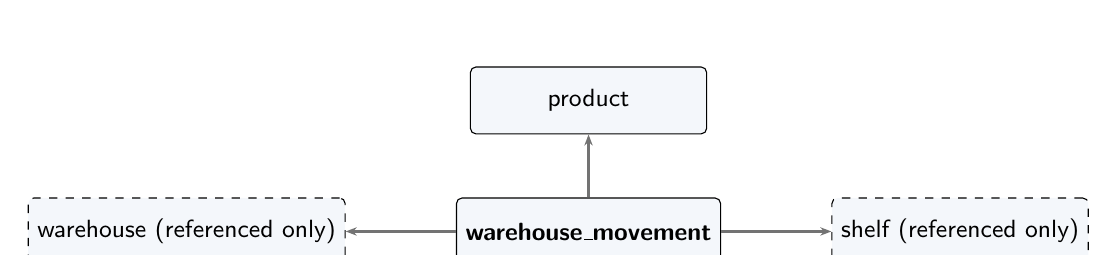
\begin{tikzpicture}[
  entity/.style={draw, rounded corners=2pt, minimum width=3.0cm, minimum height=0.85cm, align=center, font=\small\sffamily, fill=nodefill},
  arr/.style={-{Stealth[length=4pt]}, thick, black!55}
]
  \node[entity] (move) {\textbf{warehouse\_movement}};
  \node[entity, above=0.8cm of move] (prod) {product};
  \node[entity, left=1.4cm of move, draw, dashed] (wh) {warehouse (referenced only)};
  \node[entity, right=1.4cm of move, draw, dashed] (shelf) {shelf (referenced only)};
  \draw[arr] (move) -- (prod);
  \draw[arr] (move) -- (wh);
  \draw[arr] (move) -- (shelf);
\end{tikzpicture}
\caption{Inventory domain. A single table
\texttt{warehouse\_movement} records every movement of stock
(in, out, transfer). \texttt{warehouse} and \texttt{shelf}
are referenced by ID but have no master table in this dump.}
\label{fig:inventory}
\end{figure}

The \texttt{warehouse\_movement} table records:
\texttt{product\_id}, \texttt{warehouse\_id},
\texttt{shelf\_id}, \texttt{batch\_number}, \texttt{unit},
\texttt{weight}, \texttt{qty}, \texttt{movement} (the type
of movement), \texttt{rotation} (likely FIFO/LIFO/FEFO),
\texttt{barcode\_number}, \texttt{barcode\_type},
\texttt{date\_leave}, \texttt{date\_expiration}, plus the
standard \texttt{date\_added}/\texttt{date\_modified}.
This is a complete batch-and-expiry inventory movement log,
suitable for food, pharmaceuticals or any regulated goods
where traceability matters.

\subsection{Domain 10 --- Tax and Geography}\label{sec:tax}

\begin{figure}[htbp]
\centering
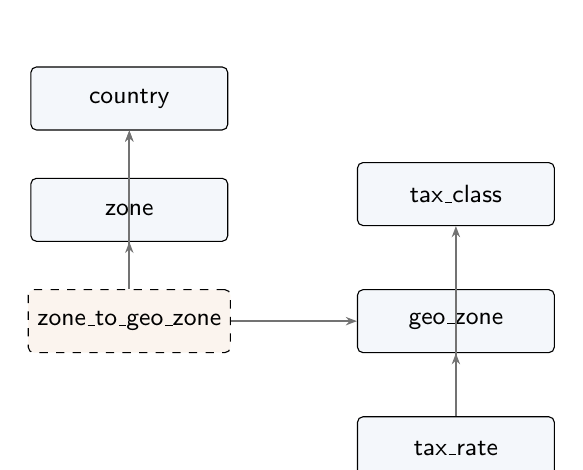
\begin{tikzpicture}[
  entity/.style={draw, rounded corners=2pt, minimum width=2.5cm, minimum height=0.8cm, align=center, font=\small\sffamily, fill=nodefill},
  junction/.style={draw, rounded corners=2pt, minimum width=2.5cm, minimum height=0.8cm, align=center, font=\small\sffamily, fill=nodefillalt, dashed},
  arr/.style={-{Stealth[length=4pt]}, thick, black!55}
]
  \node[entity] (country) {country};
  \node[entity, below=0.6cm of country] (zone) {zone};
  \node[junction, below=0.6cm of zone] (z2gz) {zone\_to\_geo\_zone};
  \node[entity, right=1.6cm of z2gz] (gz) {geo\_zone};
  \node[entity, above=0.8cm of gz] (taxc) {tax\_class};
  \node[entity, below=0.8cm of gz] (taxr) {tax\_rate};

  \draw[arr] (zone) -- (country);
  \draw[arr] (z2gz) -- (zone);
  \draw[arr] (z2gz) -- (country);
  \draw[arr] (z2gz) -- (gz);
  \draw[arr] (taxr) -- (gz);
  \draw[arr] (taxr) -- (taxc);
\end{tikzpicture}
\caption{Tax and geography ERD. Countries contain zones (states/
provinces). Zones (or whole countries) are grouped into
\texttt{geo\_zone}s via \texttt{zone\_to\_geo\_zone}. Each
\texttt{tax\_rate} applies within a \texttt{geo\_zone} and
belongs to a \texttt{tax\_class}. The catalog
(\texttt{product.tax\_class\_id}) references
\texttt{tax\_class}. This is the standard OpenCart tax model.}
\label{fig:tax}
\end{figure}

The tax/geography domain is exactly OpenCart's. Countries have
ISO codes (\texttt{iso\_code\_2}, \texttt{iso\_code\_3}) and
an \texttt{address\_format} template. Zones belong to countries.
A many-to-many \texttt{zone\_to\_geo\_zone} table groups zones
into ``geo zones'' for tax-rule purposes (e.g.\ ``Andean
region'', ``Caribbean region''). \texttt{tax\_class} groups
related tax rates (e.g.\ ``Taxable Goods''). \texttt{tax\_rate}
defines a rate, scoped to a geo zone, with a priority. The
application computes the applicable tax for a cart by looking
up the customer's shipping zone, finding the matching geo
zones, finding the tax rates for the products' tax classes
within those geo zones, and applying them in priority order.

\subsection{Domain 11 --- Users, Groups and Audit}\label{sec:users}

\begin{figure}[htbp]
\centering
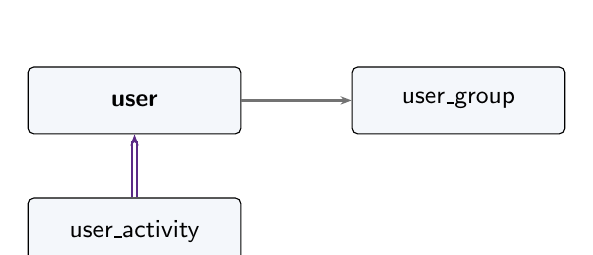
\begin{tikzpicture}[
  entity/.style={draw, rounded corners=2pt, minimum width=2.7cm, minimum height=0.85cm, align=center, font=\small\sffamily, fill=nodefill},
  arr/.style={-{Stealth[length=4pt]}, thick, black!55},
  parr/.style={-{Stealth[length=4pt]}, thick, necoyoad-purple, double, double distance=1pt}
]
  \node[entity] (user) {\textbf{user}};
  \node[entity, right=1.4cm of user] (ugroup) {user\_group};
  \node[entity, below=0.8cm of user] (uact) {user\_activity};
  \draw[arr] (user) -- (ugroup);
  \draw[parr] (uact) -- (user);
\end{tikzpicture}
\caption{User/permission domain. Admin \texttt{user}s belong to
a \texttt{user\_group} whose \texttt{permission} column is a
serialised PHP structure of allowed \texttt{route=...} patterns.
The \texttt{user\_activity} table is a polymorphic audit log
(recorded against any \texttt{object\_id/object\_type}).}
\label{fig:users}
\end{figure}

The \texttt{user} table is the admin-staff account table
(distinct from \texttt{customer}, which is the storefront
account). Each user has a \texttt{user\_group\_id} whose
\texttt{permission} column is a \texttt{TEXT} blob. The
content of this blob, by OpenCart convention, is a
serialised PHP associative array with two keys,
\texttt{access} and \texttt{modify}, each containing a list
of \texttt{catalog/*} or \texttt{admin/*} route patterns the
group is allowed to access or modify. The front controller
checks the current user's group \texttt{permission} against
the requested route before dispatching.

The \texttt{user\_activity} table is the admin audit log.
Each row records: \texttt{user\_id}, the polymorphic
\texttt{object\_id}/\texttt{object\_type} pair, an
\texttt{event} (e.g.\ \texttt{login}, \texttt{logout},
\texttt{add}, \texttt{edit}, \texttt{delete}), an
\texttt{action}, a free-text \texttt{description}, the
\texttt{ip}, \texttt{browser}, \texttt{browser\_version},
\texttt{os}, \texttt{session} (serialised), and a timestamp.
This is the same HTTP-context snapshot pattern as the
marketing and stats tables.

\subsection{Domain 12 --- Tasks and Scheduler}\label{sec:tasks}

\begin{figure}[htbp]
\centering
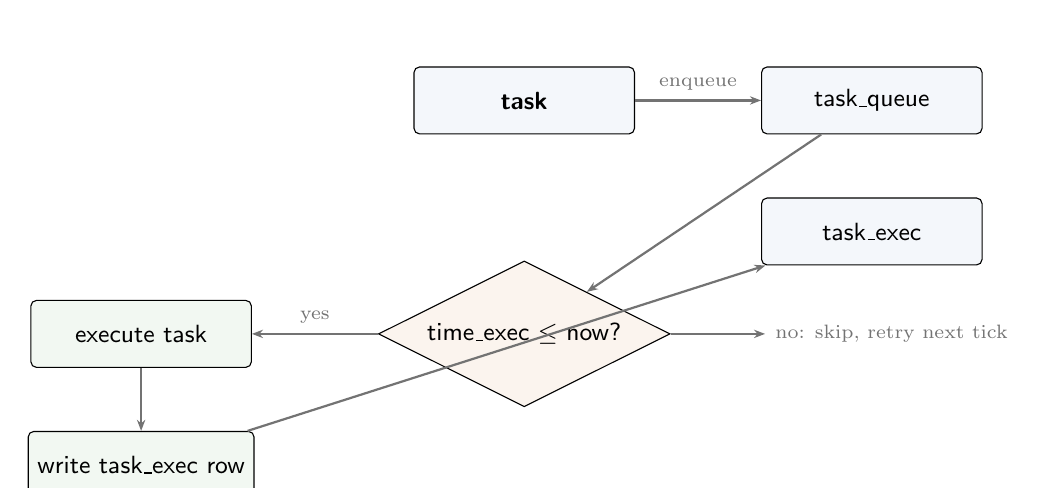
\begin{tikzpicture}[
  entity/.style={draw, rounded corners=2pt, minimum width=2.8cm, minimum height=0.85cm, align=center, font=\small\sffamily, fill=nodefill},
  decision/.style={draw, diamond, aspect=2, minimum width=2.2cm, align=center, font=\small\sffamily, fill=nodefillalt},
  arr/.style={-{Stealth[length=4pt]}, thick, black!55}
]
  \node[entity] (task) {\textbf{task}};
  \node[entity, right=1.6cm of task] (tq) {task\_queue};
  \node[entity, below=0.8cm of tq] (te) {task\_exec};
  \node[decision, below=1.6cm of task] (dec) {time\_exec \(\leq\) now?};
  \node[entity, left=1.6cm of dec, fill=nodefillgreen] (run) {execute task};
  \node[entity, below=0.8cm of run, fill=nodefillgreen] (done) {write task\_exec row};

  \draw[arr] (task) -- node[font=\scriptsize,above] {enqueue} (tq);
  \draw[arr] (tq) -- (dec);
  \draw[arr] (dec) -- node[font=\scriptsize,above] {yes} (run);
  \draw[arr] (run) -- (done);
  \draw[arr] (done) -- (te);
  \draw[arr] (dec.east) -- ++(1.2,0) node[font=\scriptsize,right] {no: skip, retry next tick} ;
\end{tikzpicture}
\caption{Task scheduler. The \texttt{task} table holds the
template (what to run, on what cadence). The
\texttt{task\_queue} table holds the materialised,
parameterised instances waiting to run. The
\texttt{task\_exec} table is the audit log of past
executions. The runner (cron or pseudo-cron) polls
\texttt{task\_queue} for rows whose \texttt{time\_exec} has
passed, executes them, and writes a \texttt{task\_exec} row.}
\label{fig:tasks}
\end{figure}

The \texttt{task} table records: \texttt{store\_id},
\texttt{object\_id}/\texttt{object\_type} (the entity the task
operates on), \texttt{task} (a name identifying the task
handler), \texttt{type}, \texttt{params} (serialised), the
schedule (\texttt{time\_interval}, \texttt{time\_exec},
\texttt{time\_last\_exec}, \texttt{run\_once}),
\texttt{status}, \texttt{sort\_order}, and execution-window
columns (\texttt{date\_start\_exec}, \texttt{date\_end\_exec}).
Note the typo \texttt{data\_added} (instead of
\texttt{date\_added}) --- a small but real artifact of the
system's hand-built evolution.

The \texttt{task\_queue} table is the per-instance queue:
\texttt{task\_id}, \texttt{params} (per-run parameters, can
override the task template's), \texttt{time\_exec} (when to
run), \texttt{status}, \texttt{sort\_order}. The
\texttt{task\_exec} table records: \texttt{task\_id},
\texttt{type}, \texttt{status}, \texttt{date\_added}. The
runner picks up due rows, runs them, writes a \texttt{task\_exec}
row, and updates the \texttt{task\_queue} row's status.

The marketing-campaign subsystem uses this scheduler directly:
each \texttt{campaign\_contact} row references a
\texttt{task\_queue\_id}, so the campaign send is literally a
queue of tasks, one per recipient.

\subsection{Domain 13 --- Localisation}\label{sec:l10n}

\begin{figure}[htbp]
\centering
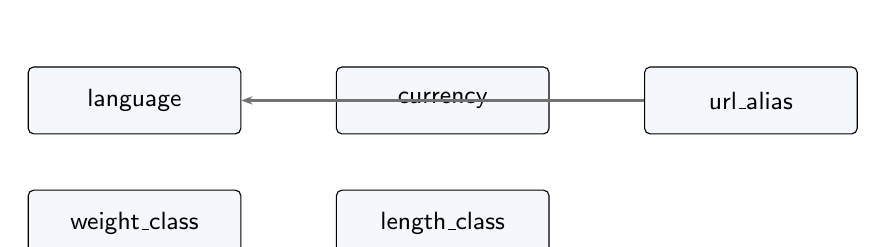
\begin{tikzpicture}[
  entity/.style={draw, rounded corners=2pt, minimum width=2.7cm, minimum height=0.85cm, align=center, font=\small\sffamily, fill=nodefill},
  arr/.style={-{Stealth[length=4pt]}, thick, black!55}
]
  \node[entity] (lang) {language};
  \node[entity, right=1.2cm of lang] (cur) {currency};
  \node[entity, below=0.7cm of lang] (wcl) {weight\_class};
  \node[entity, below=0.7cm of cur] (lcl) {length\_class};
  \node[entity, right=1.2cm of cur] (url) {url\_alias};
  \draw[arr] (url) -- (lang);
\end{tikzpicture}
\caption{Localisation domain. The four unit-class tables
(language, currency, weight\_class, length\_class) are
reference lookups. The \texttt{url\_alias} table is the SEO
layer: it maps human-readable keywords to internal
\texttt{(object\_id, object\_type, language\_id)} triples.}
\label{fig:l10n}
\end{figure}

\subsubsection{Language}

The \texttt{language} table is small but expressive:
\texttt{name}, \texttt{code} (e.g.\ ``en-gb'', ``es-ve''),
\texttt{locale} (a full locale string), \texttt{image} (a
flag icon path), \texttt{directory} and \texttt{filename}
(the PHP language file to load). This last pair is the
OpenCart convention: translations live in
\texttt{catalog/language/<directory>/<filename>.php} and are
loaded into a \texttt{\$\_} array at request startup.

\subsubsection{Currency}

The \texttt{currency} table records each currency's
\texttt{code}, \texttt{symbol\_left}, \texttt{symbol\_right},
\texttt{decimal\_place}, and \texttt{value} (the exchange
rate relative to the base currency). The
\texttt{date\_modified} column on \texttt{currency} is the
last time the rate was updated. There is no built-in
auto-update mechanism; the application either polls an
external rate service via a task, or expects an admin to
update rates manually.

\subsubsection{\texttt{url\_alias} --- The SEO Layer}

The \texttt{url\_alias} table is the system's SEO-URL layer.
Each row maps a \texttt{keyword} (the slug, e.g.\
``my-first-product'') to an internal \texttt{query} string
(e.g.\ \texttt{product\_id=42}), scoped by
\texttt{object\_id}, \texttt{object\_type} and
\texttt{language\_id}. Two unique keys enforce correctness:
\texttt{keyword + language\_id} must be unique (so the same
slug cannot point to two objects in the same language), and
\texttt{object\_id + language\_id + object\_type} must be
unique (so each object has at most one slug per language).
This is a polymorphic, language-aware short-URL system ---
see Section~\ref{sec:seo} for the routing algorithm.

\subsection{Domain 14 --- Notifications, Stats and Search}\label{sec:audit}

\begin{figure}[htbp]
\centering
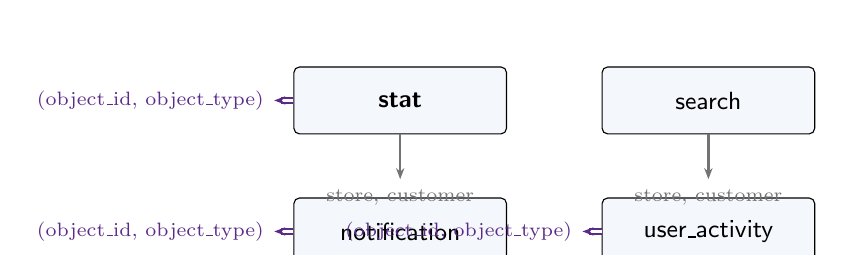
\begin{tikzpicture}[
  entity/.style={draw, rounded corners=2pt, minimum width=2.7cm, minimum height=0.85cm, align=center, font=\small\sffamily, fill=nodefill},
  arr/.style={-{Stealth[length=4pt]}, thick, black!55},
  parr/.style={-{Stealth[length=4pt]}, thick, necoyoad-purple, double, double distance=1pt}
]
  \node[entity] (stat) {\textbf{stat}};
  \node[entity, right=1.2cm of stat] (search) {search};
  \node[entity, below=0.8cm of stat] (notif) {notification};
  \node[entity, below=0.8cm of search] (uact) {user\_activity};
  \draw[parr] (stat) -- ++(-1.6,0) node[font=\scriptsize,left] {(object\_id, object\_type)};
  \draw[arr] (stat) -- ++(0,-1.0) node[font=\scriptsize,below] {store, customer};
  \draw[arr] (search) -- ++(0,-1.0) node[font=\scriptsize,below] {store, customer};
  \draw[parr] (notif) -- ++(-1.6,0) node[font=\scriptsize,left] {(object\_id, object\_type)};
  \draw[parr] (uact) -- ++(-1.6,0) node[font=\scriptsize,left] {(object\_id, object\_type)};
\end{tikzpicture}
\caption{Audit and analytics domain. Four tables record
per-request or per-action events: \texttt{stat} (page views),
\texttt{search} (search queries), \texttt{notification}
(admin/customer notifications), \texttt{user\_activity}
(admin audit log). All four carry a polymorphic
\texttt{(object\_id, object\_type)} reference, and three
(\texttt{stat}, \texttt{search}, \texttt{user\_activity})
carry a full HTTP-context snapshot.}
\label{fig:audit}
\end{figure}

The audit/analytics domain is implemented as four independent
event-log tables, all following the same general shape:

\begin{itemize}[leftmargin=1.6em,itemsep=2pt]
  \item \texttt{stat} --- a row per page view, recording the
        \texttt{customer\_id}, the polymorphic object being
        viewed, the \texttt{store\_id}/\texttt{store\_url},
        the full HTTP context (\texttt{server}, \texttt{session},
        \texttt{request}, \texttt{ref}), the user-agent
        details (\texttt{browser}, \texttt{browser\_version},
        \texttt{os}), the \texttt{ip}, and a timestamp. The
        \texttt{email} column hints that the application
        tries to attribute anonymous views to an email
        address when possible.
  \item \texttt{search} --- a row per search query, recording
        the \texttt{urlQuery} (the search string and filters),
        the customer, the store, and the same HTTP context.
  \item \texttt{notification} --- a per-user notification,
        polymorphic on the object that triggered it. Has a
        \texttt{message} column (described in the SQL comment
        as ``Mensaje que sera traducido'' --- a message that
        will be translated, i.e.\ a translation key with
        parameters), a \texttt{url} for the user to click
        through to, and a \texttt{type}.
  \item \texttt{user\_activity} --- the admin audit log,
        described in Section~\ref{sec:users}.
\end{itemize}

The four tables are clearly part of the same conceptual
family (per-event analytics with full HTTP context) but use
slightly different column sets, suggesting they were added
at different times by different code paths.

\subsection{Domain 15 --- Settings and Extensions}\label{sec:settings}

\begin{figure}[htbp]
\centering
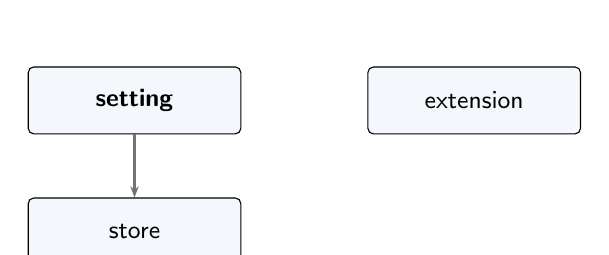
\begin{tikzpicture}[
  entity/.style={draw, rounded corners=2pt, minimum width=2.7cm, minimum height=0.85cm, align=center, font=\small\sffamily, fill=nodefill},
  arr/.style={-{Stealth[length=4pt]}, thick, black!55}
]
  \node[entity] (setting) {\textbf{setting}};
  \node[entity, right=1.6cm of setting] (ext) {extension};
  \node[entity, below=0.8cm of setting] (store) {store};
  \draw[arr] (setting) -- (store);
\end{tikzpicture}
\caption{Configuration domain. The \texttt{setting} table is a
flat key-value store, scoped by \texttt{store\_id} and
\texttt{group}. The \texttt{extension} table is a registry of
installed extensions (payment, shipping, total, payment-report,
etc.) with licensing metadata.}
\label{fig:settings}
\end{figure}

\subsubsection{The Flat Settings Store}

The \texttt{setting} table is OpenCart's classic flat
configuration store: each row is a (\texttt{store\_id},
\texttt{group}, \texttt{key}, \texttt{value}) tuple. A row
with \texttt{store\_id = 0} is the default; rows with
\texttt{store\_id = N > 0} override the default for that
store. The \texttt{group} typically names the extension
(e.g.\ ``config'', ``shipping\_flat'',
\texttt{payment\_bank\_transfer}); the \texttt{key} is the
parameter name (e.g.\ ``geocode'', ``telephone'',
``flat\_cost''); the \texttt{value} is a string. The
application loads all settings for the current store at
request startup and caches them in a registry.

\subsubsection{Extensions}

The \texttt{extension} table is the registry of installed
extensions. It is significantly richer than vanilla
OpenCart's. Columns: \texttt{type} (the extension category:
\texttt{payment}, \texttt{shipping}, \texttt{total},
\texttt{module}, \texttt{feed}, \texttt{analytics},
\texttt{report}, ...), \texttt{app} (which app:
\texttt{catalog} or \texttt{admin}), \texttt{key} (the
extension's unique code), \texttt{license} (a license key),
\texttt{install} and \texttt{uninstall} (URLs or controller
routes for installation / uninstallation hooks),
\texttt{url\_developer} (the developer's website),
\texttt{settings} (serialised extension-specific settings),
\texttt{version}, \texttt{status}, \texttt{last\_update},
\texttt{date\_added}. The presence of \texttt{license},
\texttt{install}, \texttt{uninstall} and
\texttt{url\_developer} strongly suggests a commercial
extension marketplace: extensions can be bought, licensed,
installed and uninstalled from the admin UI.

% ============================================================
\section{Cross-Cutting Patterns, Formalised}\label{sec:crosscutting}
% ============================================================

Section~\ref{sec:style} introduced the four cross-cutting patterns
in prose. Here we formalise them with a single combined diagram and
an inventory of every table that participates in each.

\subsection{Pattern Map}

\begin{figure}[htbp]
\centering
\resizebox{\columnwidth}{!}{%
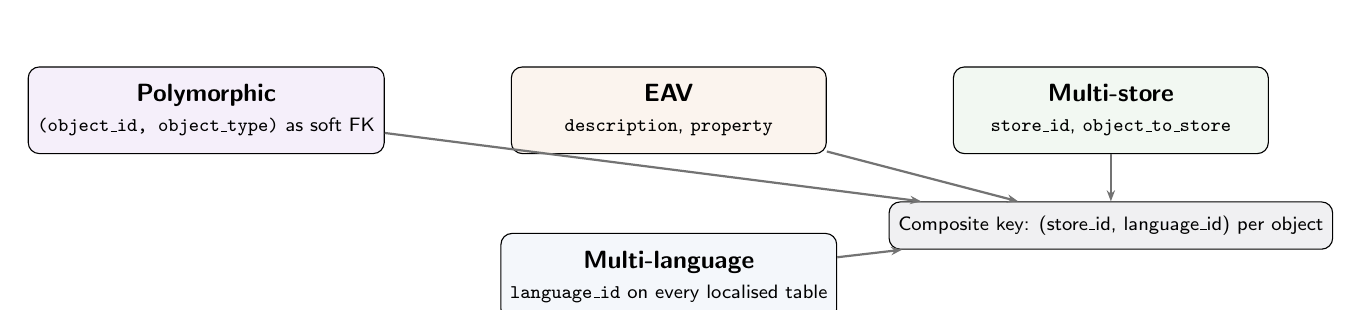
\begin{tikzpicture}[
  pat/.style={draw, rounded corners=4pt, minimum width=4.0cm, minimum height=1.1cm, align=center, font=\small\sffamily, fill=nodefill},
  arr/.style={-{Stealth[length=4pt]}, thick, black!55}
]
  \node[pat, fill=nodefillpurple] (p1) {\textbf{Polymorphic}\\\scriptsize \texttt{(object\_id, object\_type)} as soft FK};
  \node[pat, fill=nodefillalt, right=1.6cm of p1] (p2) {\textbf{EAV}\\\scriptsize \texttt{description}, \texttt{property}};
  \node[pat, fill=nodefillgreen, right=1.6cm of p2] (p3) {\textbf{Multi-store}\\\scriptsize \texttt{store\_id}, \texttt{object\_to\_store}};
  \node[pat, fill=nodefill, below=1.0cm of p2] (p4) {\textbf{Multi-language}\\\scriptsize \texttt{language\_id} on every localised table};

  \node[draw, rounded corners=4pt, below=0.6cm of p3, minimum width=4.0cm, minimum height=0.6cm, fill=nodefillgray, font=\scriptsize\sffamily] (composite) {Composite key: (store\_id, language\_id) per object};
  \draw[arr] (p1) -- (composite);
  \draw[arr] (p2) -- (composite);
  \draw[arr] (p3) -- (composite);
  \draw[arr] (p4) -- (composite);
\end{tikzpicture}%
}
\caption{The four cross-cutting patterns compose. A single piece
of content --- say, a product's Spanish description shown on
Store 2 --- is located by the composite key
\texttt{(store\_id=2, language\_id=2, object\_id=42,
object\_type='product')}.}
\label{fig:patterns}
\end{figure}

\subsection{Polymorphic Association Inventory}

\small
\begin{longtable}{>{\raggedright\arraybackslash}p{4.2cm}>{\raggedright\arraybackslash}p{4.4cm}>{\raggedright\arraybackslash}p{6.0cm}}
\caption{Every polymorphic \texttt{(object\_id, object\_type)} association in the schema.}\label{tab:polymorphic}\\
\toprule
\textbf{Table} & \textbf{Polymorphic columns} & \textbf{What it points to} \\
\midrule
\endfirsthead
\toprule
\textbf{Table} & \textbf{Polymorphic columns} & \textbf{What it points to} \\
\midrule
\endhead
\bottomrule
\endfoot
\texttt{object}                 & \texttt{parent\_id}, \texttt{parent\_type}             & any other object (tree support) \\
\texttt{object\_to\_category}   & \texttt{object\_id}, \texttt{object\_type}             & any object to a category \\
\texttt{object\_to\_store}      & \texttt{object\_id}, \texttt{object\_type}             & any object to a store \\
\texttt{description}            & \texttt{object\_id}, \texttt{object\_type}             & any object's localised text \\
\texttt{property}               & \texttt{object\_id}, \texttt{object\_type}             & any object's free-form key-value \\
\texttt{url\_alias}             & \texttt{object\_id}, \texttt{object\_type}             & any object's SEO slug \\
\texttt{review}                 & \texttt{object\_id}, \texttt{object\_type}             & any object's review \\
\texttt{review\_likes}          & \texttt{object\_id}, \texttt{object\_type}             & the review's parent object \\
\texttt{stat}                   & \texttt{object\_id}, \texttt{object\_type}             & the object being viewed \\
\texttt{notification}           & \texttt{object\_id}, \texttt{object\_type}             & the object that triggered the notification \\
\texttt{user\_activity}         & \texttt{object\_id}, \texttt{object\_type}             & the object the admin acted on \\
\texttt{task}                   & \texttt{object\_id}, \texttt{object\_type}             & the object the task operates on \\
\texttt{widget\_landing\_page}  & \texttt{object\_type}                                  & the type of landing page \\
\texttt{category}               & \texttt{object\_type}                                  & the kind of object the category groups \\
\texttt{campaign\_link\_stat}   & \texttt{(implicit via contact + campaign)}            & marketing context \\
\texttt{campaign\_stat}         & \texttt{(implicit via contact + campaign)}            & marketing context \\
\end{longtable}

\subsection{The ``params'' / ``settings'' Escape Hatch}

At least seven tables carry a \texttt{TEXT} column whose payload
is a serialised PHP value: \texttt{object.params},
\texttt{banner.params}, \texttt{customer\_group.params},
\texttt{extension.settings}, \texttt{widget.settings},
\texttt{setting.value} (sometimes), \texttt{task.params},
\texttt{task\_queue.params}, \texttt{product\_attribute.params}
(not present, but \texttt{property.value} plays the same role).
This is a deliberate, schema-level escape hatch: anything that
does not fit the relational model is stuffed into a
serialised blob and decoded in PHP. The cost is opacity: from
the SQL side, one cannot query, index or join on the contents
of these blobs. They are a frequent source of bugs when the
serialised format changes between PHP versions (e.g.\ PHP 7's
\texttt{serialize()} of \texttt{C}losure objects differs from
PHP 8's).

\subsection{Composite Conventions}

Three column-pair conventions are stable across the schema:

\begin{itemize}[leftmargin=1.6em,itemsep=2pt]
  \item \texttt{date\_added} + \texttt{date\_modified}: present on
        virtually every entity table. Some use \texttt{TIMESTAMP
        DEFAULT CURRENT\_TIMESTAMP} for \texttt{date\_added};
        others use \texttt{DATETIME} with a default of
        \texttt{'0000-00-00 00:00:00'}. The mix is a tell-tale
        of organic growth --- different tables were added at
        different times.
  \item \texttt{status} + \texttt{sort\_order}: present on most
        entity and lookup tables. The \texttt{status} semantics
        vary (see Section~\ref{sec:style}); \texttt{sort\_order}
        is a manual display-ordering integer.
  \item \texttt{store\_id} (optional): present when an entity is
        store-scoped. The convention is that \texttt{store\_id = 0}
        means ``all stores'' or ``default store''; non-zero values
        mean ``this specific store only''.
\end{itemize}

% ============================================================
\section{Inferred HTTP Request Lifecycle}\label{sec:lifecycle}
% ============================================================

Although the PHP source is not in the repository, the OpenCart
convention is rigid enough that we can reconstruct the request
lifecycle with high confidence. The schema provides several direct
signals: the \texttt{url\_alias} table (the routing layer), the
\texttt{stat} table (page-view logging), the \texttt{setting}
table (configuration loading), the \texttt{language} table
(translation loading), and the \texttt{widget} table (layout
assembly).

\begin{figure}[htbp]
\centering
\resizebox{\columnwidth}{!}{%
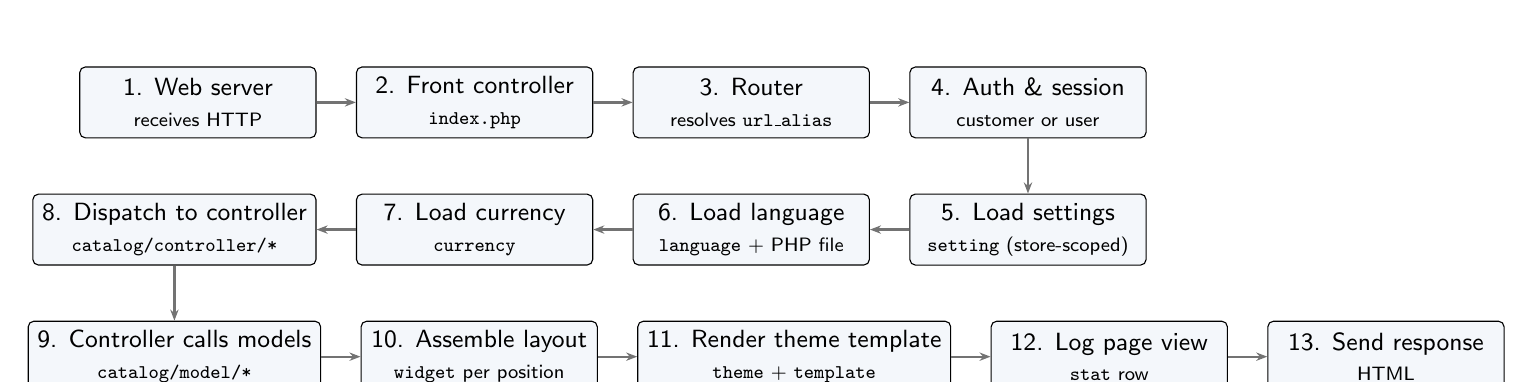
\begin{tikzpicture}[
  phase/.style={draw, rounded corners=2pt, minimum width=3.0cm, minimum height=0.9cm, align=center, font=\small\sffamily, fill=nodefill},
  arr/.style={-{Stealth[length=4pt]}, thick, black!55}
]
  \node[phase] (p1) {1. Web server\\\scriptsize receives HTTP};
  \node[phase, right=0.5cm of p1] (p2) {2. Front controller\\\scriptsize \texttt{index.php}};
  \node[phase, right=0.5cm of p2] (p3) {3. Router\\\scriptsize resolves \texttt{url\_alias}};
  \node[phase, right=0.5cm of p3] (p4) {4. Auth \& session\\\scriptsize customer or user};
  \node[phase, below=0.7cm of p4] (p5) {5. Load settings\\\scriptsize \texttt{setting} (store-scoped)};
  \node[phase, left=0.5cm of p5] (p6) {6. Load language\\\scriptsize \texttt{language} + PHP file};
  \node[phase, left=0.5cm of p6] (p7) {7. Load currency\\\scriptsize \texttt{currency}};
  \node[phase, left=0.5cm of p7] (p8) {8. Dispatch to controller\\\scriptsize \texttt{catalog/controller/*}};
  \node[phase, below=0.7cm of p8] (p9) {9. Controller calls models\\\scriptsize \texttt{catalog/model/*}};
  \node[phase, right=0.5cm of p9] (p10) {10. Assemble layout\\\scriptsize \texttt{widget} per position};
  \node[phase, right=0.5cm of p10] (p11) {11. Render theme template\\\scriptsize \texttt{theme} + \texttt{template}};
  \node[phase, right=0.5cm of p11] (p12) {12. Log page view\\\scriptsize \texttt{stat} row};
  \node[phase, right=0.5cm of p12] (p13) {13. Send response\\\scriptsize HTML};

  \draw[arr] (p1) -- (p2);
  \draw[arr] (p2) -- (p3);
  \draw[arr] (p3) -- (p4);
  \draw[arr] (p4) -- (p5);
  \draw[arr] (p5) -- (p6);
  \draw[arr] (p6) -- (p7);
  \draw[arr] (p7) -- (p8);
  \draw[arr] (p8) -- (p9);
  \draw[arr] (p9) -- (p10);
  \draw[arr] (p10) -- (p11);
  \draw[arr] (p11) -- (p12);
  \draw[arr] (p12) -- (p13);
\end{tikzpicture}%
}
\caption{Inferred HTTP request lifecycle. The 13 phases reconstruct
the standard OpenCart-derived front-controller pipeline. The schema
touches the database at phases 3 (URL alias), 4 (session/customer),
5 (settings), 6 (language), 7 (currency), 8 (dispatch --- the
permission check on \texttt{user\_group.permission}), 9 (model
queries), 10 (widgets), 11 (theme), and 12 (stat).}
\label{fig:lifecycle}
\end{figure}

\subsection{Phase Notes}

\begin{description}[leftmargin=1.6em,itemsep=2pt,font=\bfseries\small]
  \item[Phase 3 --- Router:] The router first checks
        \texttt{url\_alias} for a slug matching the request path
        and the current \texttt{language\_id}. If found, it
        reconstructs the internal \texttt{route=controller/method}
        string. If not found, it falls back to the query string
        \texttt{?route=...}. See Section~\ref{sec:seo} for the
        full algorithm.
  \item[Phase 4 --- Auth:] The session is loaded. If the customer
        is logged in, the \texttt{customer} row is fetched and
        cached. The visit counter (\texttt{customer.visits}) is
        incremented and the IP is updated. If the admin is
        logged in (admin route), the \texttt{user} row is fetched
        and the \texttt{user\_group.permission} blob is decoded.
  \item[Phase 5 --- Settings:] All rows from \texttt{setting}
        with \texttt{store\_id = 0} (defaults) and
        \texttt{store\_id = current\_store\_id} (overrides) are
        loaded. The overrides win. The result is a flat
        \texttt{config} array.
  \item[Phase 6 --- Language:] The \texttt{language} row for the
        current language is loaded. The PHP file
        \texttt{catalog/language/<directory>/<filename>.php} is
        included; it populates a \texttt{\$\_} array of
        translation strings.
  \item[Phase 8 --- Dispatch:] The front controller instantiates
        the target \texttt{Controller} class and calls the target
        method. For admin routes, the user's
        \texttt{user\_group.permission} is checked against the
        route. If the route is not in the \texttt{access} or
        \texttt{modify} list, the request is denied.
  \item[Phase 10 --- Layout:] The \texttt{widget} table is queried
        for widgets in the current store, position, landing page,
        and object type, sorted by \texttt{order}. Each widget's
        \texttt{extension} is loaded, its \texttt{settings} are
        decoded, and the widget controller is invoked to render
        into the layout position.
  \item[Phase 12 --- Stat:] A row is inserted into \texttt{stat}
        recording the page view, with the full HTTP context.
\end{description}

% ============================================================
\section{Inferred Customer Checkout Flow}\label{sec:checkout}
% ============================================================

\begin{figure}[htbp]
\centering
\resizebox{\columnwidth}{!}{%
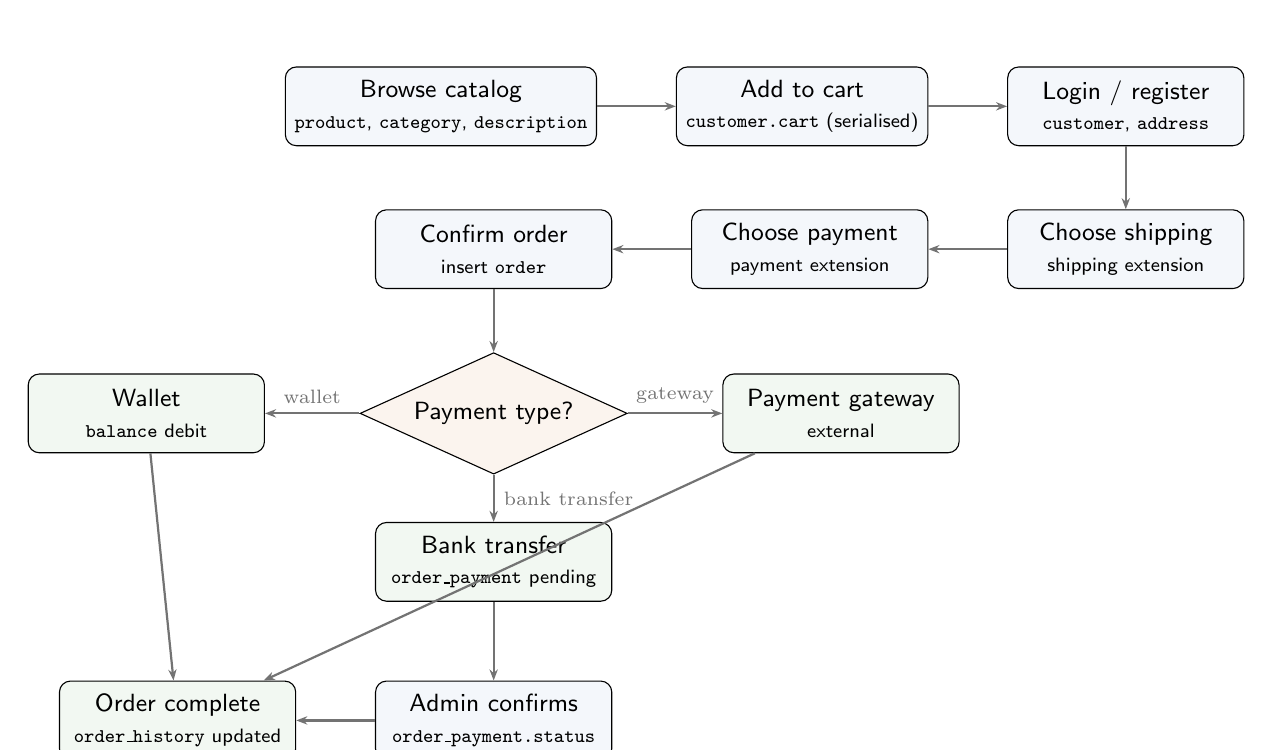
\begin{tikzpicture}[
  state/.style={draw, rounded corners=4pt, minimum width=3.0cm, minimum height=1.0cm, align=center, font=\small\sffamily, fill=nodefill},
  decision/.style={draw, diamond, aspect=2.2, align=center, font=\small\sffamily, fill=nodefillalt},
  arr/.style={-{Stealth[length=4pt]}, thick, black!55}
]
  \node[state] (browse) {Browse catalog\\\scriptsize \texttt{product}, \texttt{category}, \texttt{description}};
  \node[state, right=1.0cm of browse] (cart)  {Add to cart\\\scriptsize \texttt{customer.cart} (serialised)};
  \node[state, right=1.0cm of cart]   (login) {Login / register\\\scriptsize \texttt{customer}, \texttt{address}};
  \node[state, below=0.8cm of login]  (ship)  {Choose shipping\\\scriptsize shipping extension};
  \node[state, left=1.0cm of ship]    (pay)   {Choose payment\\\scriptsize payment extension};
  \node[state, left=1.0cm of pay]     (confirm) {Confirm order\\\scriptsize insert \texttt{order}};
  \node[decision, below=0.8cm of confirm] (dec) {Payment type?};
  \node[state, left=1.2cm of dec, fill=nodefillgreen] (wallet) {Wallet\\\scriptsize \texttt{balance} debit};
  \node[state, below=0.6cm of dec, fill=nodefillgreen] (bank)  {Bank transfer\\\scriptsize \texttt{order\_payment} pending};
  \node[state, right=1.2cm of dec, fill=nodefillgreen] (gateway) {Payment gateway\\\scriptsize external};
  \node[state, below=1.0cm of bank] (admin) {Admin confirms\\\scriptsize \texttt{order\_payment.status}};
  \node[state, left=1.0cm of admin, fill=nodefillgreen] (done)  {Order complete\\\scriptsize \texttt{order\_history} updated};

  \draw[arr] (browse)  -- (cart);
  \draw[arr] (cart)    -- (login);
  \draw[arr] (login)   -- (ship);
  \draw[arr] (ship)    -- (pay);
  \draw[arr] (pay)     -- (confirm);
  \draw[arr] (confirm) -- (dec);
  \draw[arr] (dec)     -- node[font=\scriptsize, above] {wallet} (wallet);
  \draw[arr] (dec)     -- node[font=\scriptsize, right] {bank transfer} (bank);
  \draw[arr] (dec)     -- node[font=\scriptsize, above] {gateway} (gateway);
  \draw[arr] (bank)    -- (admin);
  \draw[arr] (admin)   -- (done);
  \draw[arr] (wallet)  -- (done);
  \draw[arr] (gateway) -- (done);
\end{tikzpicture}%
}
\caption{Inferred customer checkout flow. The cart is held in the
\texttt{customer.cart} serialised blob (for logged-in customers)
or in the PHP session (for guests). At confirmation, a row is
inserted into \texttt{order} (with snapshot fields),
\texttt{order\_product}, \texttt{order\_option},
\texttt{order\_total}, and the first \texttt{order\_history} row.
The payment path branches into three: wallet debit (immediate),
bank transfer (waits for admin confirmation), or external gateway
(callback-driven). All three converge on a final
\texttt{order\_history} status update.}
\label{fig:checkout}
\end{figure}

\subsection{Snapshot Writes at Confirmation}

At order confirmation the application performs a multi-table,
non-atomic write (MyISAM has no transactions). The order of
operations is, by OpenCart convention:

\begin{enumerate}[leftmargin=1.6em,itemsep=2pt]
  \item Insert into \texttt{order} (snapshot of customer, address,
        shipping, payment, totals, currency, language).
  \item For each cart line: insert into \texttt{order\_product}
        (snapshot of name, model, price, tax, quantity), then
        insert into \texttt{order\_option} for each selected
        option (snapshot of option name, value, price delta).
  \item For each \texttt{order\_total} line: insert into
        \texttt{order\_total}.
  \item If the product is downloadable: insert into
        \texttt{order\_download} for each download, with
        \texttt{remaining} set to the allowed download count.
  \item If a coupon was used: insert into \texttt{coupon\_history}.
  \item Insert the first \texttt{order\_history} row, with the
        initial \texttt{order\_status\_id} (typically ``pending'').
  \item If paying by wallet: insert a debit row into
        \texttt{balance}.
  \item If paying by bank transfer: insert a pending row into
        \texttt{order\_payment}.
  \item Decrement stock: for each \texttt{order\_product} line
        where \texttt{subtract = 1}, decrement
        \texttt{product.quantity} by the ordered quantity.
  \item Optionally: insert into \texttt{task\_queue} a
        confirmation-email task.
\end{enumerate}

A crash between steps leaves the database in an inconsistent
state. This is the inherent cost of the MyISAM choice
(Section~\ref{sec:engine}).

% ============================================================
\section{Inferred Task Scheduler Lifecycle}\label{sec:cron}
% ============================================================

\begin{figure}[htbp]
\centering
\resizebox{\columnwidth}{!}{%
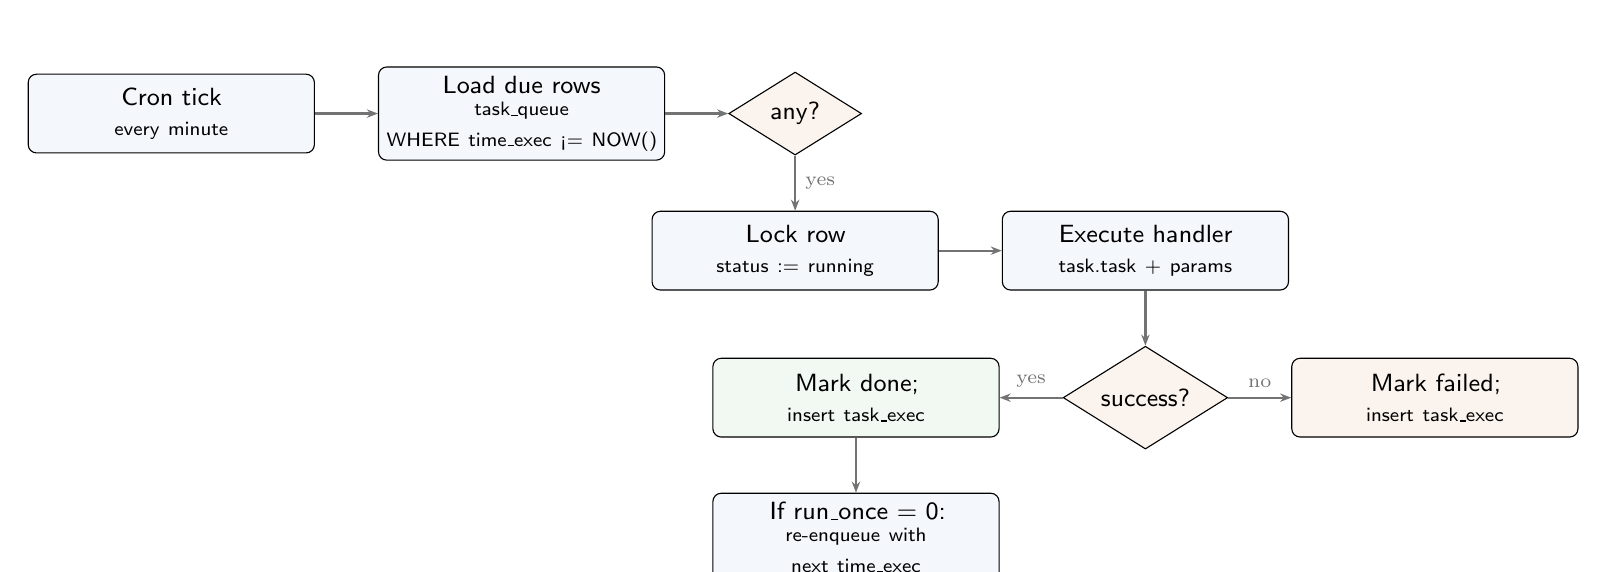
\begin{tikzpicture}[
  state/.style={draw, rounded corners=3pt, text width=3.4cm, minimum height=1.0cm, align=center, font=\small\sffamily, fill=nodefill},
  decision/.style={draw, diamond, aspect=1.6, align=center, font=\small\sffamily, fill=nodefillalt},
  arr/.style={-{Stealth[length=4pt]}, thick, black!55}
]
  \node[state] (cron) {Cron tick\\\scriptsize every minute};
  \node[state, right=0.8cm of cron] (load) {Load due rows\\\scriptsize task\_queue\\\scriptsize WHERE time\_exec <= NOW()};
  \node[decision, right=0.8cm of load] (dec1) {any?};
  \node[state, below=0.7cm of dec1] (lock) {Lock row\\\scriptsize status := running};
  \node[state, right=0.8cm of lock] (run) {Execute handler\\\scriptsize task.task + params};
  \node[decision, below=0.7cm of run] (dec2) {success?};
  \node[state, left=0.8cm of dec2, fill=nodefillgreen] (ok) {Mark done;\\\scriptsize insert task\_exec};
  \node[state, right=0.8cm of dec2, fill=nodefillalt] (fail) {Mark failed;\\\scriptsize insert task\_exec};
  \node[state, below=0.7cm of ok] (resched) {If run\_once = 0:\\\scriptsize re-enqueue with\\\scriptsize next time\_exec};

  \draw[arr] (cron) -- (load);
  \draw[arr] (load) -- (dec1);
  \draw[arr] (dec1) -- node[font=\scriptsize, right] {yes} (lock);
  \draw[arr] (lock) -- (run);
  \draw[arr] (run) -- (dec2);
  \draw[arr] (dec2) -- node[font=\scriptsize, above] {yes} (ok);
  \draw[arr] (dec2) -- node[font=\scriptsize, above] {no} (fail);
  \draw[arr] (ok) -- (resched);
\end{tikzpicture}%
}
\caption{Inferred task-scheduler tick. The runner polls the task\_queue
table for due rows, locks one, executes its handler, writes a task\_exec
audit row, and either re-enqueues (recurring) or finalises (one-shot).
The exact locking mechanism cannot be enforced by MyISAM, so the lock
is a best-effort SQL update of the row's status from pending to running.}
\label{fig:cron}
\end{figure}

\subsection{Real Cron vs.\ Pseudo-Cron}

The schema alone cannot distinguish between a real
\texttt{crontab} entry and a pseudo-cron triggered on each page
load. Two arguments favour real cron:

\begin{itemize}[leftmargin=1.6em,itemsep=2pt]
  \item The marketing subsystem enqueues per-recipient email
        sends. A pseudo-cron on page loads would tie email
        throughput to site traffic, which is unreliable.
  \item The \texttt{task\_queue.time\_exec} column implies
        precise scheduling, which only a real cron can deliver.
\end{itemize}

We therefore infer a Unix \texttt{cron} entry running every
minute, executing a PHP CLI script that performs the loop in
Figure~\ref{fig:cron}.

% ============================================================
\section{SEO and URL Routing}\label{sec:seo}
% ============================================================

The \texttt{url\_alias} table is the SEO-URL layer. Each row
maps a slug to an internal query, polymorphically and per
language. The inferred routing algorithm is:

\begin{enumerate}[leftmargin=1.6em,itemsep=2pt]
  \item \textbf{Inbound request} \texttt{GET /my-product} arrives.
  \item The front controller looks up \texttt{url\_alias} for
        \texttt{keyword = 'my-product'} AND
        \texttt{language\_id = current\_language\_id}.
  \item If found: the \texttt{query} column holds the internal
        route (e.g.\ \texttt{product\_id=42}). The router
        translates this to
        \texttt{route=product/product\&product\_id=42} and
        dispatches.
  \item If not found: the request falls through to the
        \texttt{?route=...} query-string convention, or returns
        a 404.
\end{enumerate}

Outbound, when the application generates a link to a product,
it looks up \texttt{url\_alias} for
\texttt{object\_id = 42, object\_type = 'product', language\_id = current}
and, if found, emits \texttt{/my-product} instead of
\texttt{?route=product/product\&product\_id=42}.

The two unique keys on \texttt{url\_alias} enforce correctness:

\begin{itemize}[leftmargin=1.6em,itemsep=2pt]
  \item \texttt{UNIQUE (keyword, language\_id)}: a slug is unique
        within a language. Two slugs can collide across languages.
  \item \texttt{UNIQUE (object\_id, language\_id, object\_type)}:
        each object has at most one slug per language per type.
\end{itemize}

% ============================================================
\section{Security and Permissions Model}\label{sec:security}
% ============================================================

The security model has three layers:

\subsection{Layer 1 --- Customer Authentication}

Customers authenticate with email + password (the \texttt{email}
column is unique on \texttt{customer}). The \texttt{password}
column is 100 characters wide, which fits modern hashes
(bcrypt is 60 chars, Argon2id can be up to 97). On login, the
application verifies the hash and updates \texttt{customer.ip}
and \texttt{customer.visits}. Account activation is gated by
\texttt{customer.activation\_code} (emailed at signup) and
\texttt{customer.approved} (admin-moderated). Banned customers
are blocked via \texttt{customer.banned}.

\subsection{Layer 2 --- Admin Authentication}

Admins authenticate with username + password against
\texttt{user}. The \texttt{user.password} column is also 100
characters wide. After login, the admin's
\texttt{user\_group.permission} blob is decoded and used to
gate every subsequent admin route.

\subsection{Layer 3 --- Route-Level Authorisation}

The \texttt{user\_group.permission} blob, by OpenCart
convention, has the structure:

\begin{tcolorbox}[enhanced,colback=nodefillgray,colframe=black!40,boxrule=0.3pt,arc=2pt,left=8pt,right=8pt,top=4pt,bottom=4pt,fontupper=\small\ttfamily]
array(\\
\ \ 'access' => array('catalog/product', 'catalog/category', ...),\\
\ \ 'modify' => array('catalog/product', 'catalog/category', ...)\\
)
\end{tcolorbox}

The front controller, before dispatching an admin route,
checks whether the route string is in the current user's
\texttt{access} (for GET requests) or \texttt{modify} (for
POST/PUT/DELETE requests) array. If not, the request is
denied. This is a coarse, route-level permission model ---
finer-grained permissions (per-object, per-field) are not
present in the schema.

\subsection{Audit Trail}

Every admin action is logged in \texttt{user\_activity} with
the polymorphic object reference, the event, the action, a
description, the IP and the user-agent. This is the
non-repudiation layer.

% ============================================================
\section{Data Integrity Observations}\label{sec:integrity}
% ============================================================

We repeat: this section is descriptive, not prescriptive. We
list the integrity consequences of the schema's design choices
without recommending changes.

\subsection{Consequences of MyISAM}

\begin{itemize}[leftmargin=1.6em,itemsep=2pt]
  \item No declared foreign keys. The 100+ ``\texttt{\_id}''
        columns are soft references. The application is solely
        responsible for referential integrity.
  \item No transactions. Multi-table writes (e.g.\ order
        insertion, Section~\ref{sec:checkout}) are not atomic.
  \item Table-level locking on writes. Concurrent writes to
        \texttt{stat} (one row per page view) can become a
        bottleneck on a busy site.
  \item Crashes can corrupt MyISAM tables; the schema's many
        \texttt{date\_added} and \texttt{date\_modified}
        columns help forensic recovery but cannot prevent it.
\end{itemize}

\subsection{Consequences of the Polymorphic Pattern}

\begin{itemize}[leftmargin=1.6em,itemsep=2pt]
  \item No cascade deletes. Deleting a \texttt{product} row
        leaves orphaned rows in \texttt{description},
        \texttt{property}, \texttt{url\_alias}, \texttt{review},
        \texttt{stat}, \texttt{notification},
        \texttt{user\_activity}, and \texttt{object\_to\_store}.
        The application must clean these up explicitly, or
        accept the orphans.
  \item No cascade updates. Renaming the primary key of
        \texttt{object} (impossible in practice, but
        illustrative) would not propagate.
  \item No way to enforce that an \texttt{(object\_id,
        object\_type)} pair in \texttt{description} actually
        points to a real object. A typo in
        \texttt{object\_type} silently creates an orphan.
\end{itemize}

\subsection{Consequences of the ``params'' TEXT Escape Hatch}

\begin{itemize}[leftmargin=1.6em,itemsep=2pt]
  \item The contents of \texttt{object.params},
        \texttt{banner.params}, \texttt{widget.settings},
        \texttt{extension.settings}, \texttt{task.params},
        \texttt{task\_queue.params},
        \texttt{customer\_group.params} are opaque to SQL.
  \item Schema migrations cannot change the structure of these
        blobs; the application must handle backward
        compatibility in PHP.
  \item A PHP \texttt{serialize()} / \texttt{unserialize()}
        round-trip can fail silently if the serialised object
        references a class that no longer exists or has
        changed.
\end{itemize}

\subsection{Consequences of the Snapshot Pattern}

\begin{itemize}[leftmargin=1.6em,itemsep=2pt]
  \item The \texttt{order} table is wide (43 columns) and
        deliberately denormalised. This is correct for legal
        fidelity but makes ad-hoc reporting harder.
  \item Renaming a product after an order does not affect the
        order's \texttt{order\_product.name} snapshot, which
        is the intended behaviour.
  \item The \texttt{order\_total} table stores the formatted
        \texttt{text} (e.g.\ ``USD\,120.00'') at order time.
        Currency reconfigurations do not retroactively change
        past orders.
\end{itemize}

% ============================================================
\section{Closing Observations}\label{sec:observations}
% ============================================================

We close with a set of observations that do not fit anywhere
else, and that the reader may find useful when interpreting
the rest of the document. None of these are recommendations;
they are simply features of the system that are easy to miss
on a first reading.

\subsection{The System Has Its Own Identity}

The \texttt{template.for\_nt\_version} column, the table
prefix \texttt{nts8sd4fd\_}, the absence of OpenCart's
\texttt{category\_path} table, and the presence of the
polymorphic \texttt{object} spine all indicate that
``Necoyoad'' is not a vanilla OpenCart install. It is either
a fork of OpenCart or a separate system that borrowed
OpenCart's conventions heavily. The author called the
database \texttt{necoyoad\_db}, suggesting the platform name
itself is ``Necoyoad''.

\subsection{The Venezuelan Context is Visible}

The \texttt{customer.rif} column, the \texttt{bank\_account.rif}
column, the \texttt{order\_payment} subsystem (manual bank
transfers as the primary payment method), the
\texttt{campaign.message} SQL comment in Spanish (``Mensaje que
sera traducido''), and the use of \texttt{utf8\_spanish2\_ci}
collation on the \texttt{post} table's text columns all place
the system's primary context in Venezuela. This is consistent
with the author's GitHub username (\texttt{yosietserga} is a
Latin-script rendering of a Spanish name).

\subsection{The Schema Records Its Own Evolution}

The inconsistent use of \texttt{TIMESTAMP DEFAULT CURRENT\_TIMESTAMP}
versus \texttt{DATETIME DEFAULT '0000-00-00 00:00:00'}; the
occasional typo (\texttt{data\_added} on \texttt{task}); the
mix of \texttt{latin1} default charsets with per-column
\texttt{utf8\_bin} overrides; the parallel existence of
\texttt{product\_to\_category} (specific) and
\texttt{object\_to\_category} (polymorphic) --- all of these
are the SQL-layer equivalent of growth rings. They let us
read the schema as a palimpsest of features added at different
times by different hands.

\subsection{The Marketing Subsystem is the Most Sophisticated Part}

After the catalog, the marketing subsystem
(\texttt{newsletter}, \texttt{campaign}, \texttt{contact},
\texttt{contact\_list}, \texttt{campaign\_contact},
\texttt{campaign\_link}, \texttt{campaign\_stat},
\texttt{campaign\_link\_stat}, plus the \texttt{task\_queue}
integration) is the most behaviourally complex part of the
system. It is essentially a self-hosted Mailchimp clone,
embedded in the e-commerce platform, with full open and
click tracking. This is non-trivial to build and suggests
significant investment by the author.

\subsection{The Audit Subsystem is Pervasive}

The HTTP-context snapshot pattern (\texttt{server},
\texttt{session}, \texttt{request}, \texttt{ref},
\texttt{browser}, \texttt{browser\_version}, \texttt{os},
\texttt{ip}, \texttt{date\_added}) appears in five tables:
\texttt{stat}, \texttt{search}, \texttt{user\_activity},
\texttt{campaign\_stat}, \texttt{campaign\_link\_stat}. This
is a deliberate, schema-level commitment to per-event
forensic logging. It is unusual to see this level of audit
detail in a small e-commerce platform and indicates that the
author treated analytics as a first-class concern.

% ============================================================
\section{Conclusion}\label{sec:conclusion}
% ============================================================

The Necoyoad database dump, despite being a single 76-kilobyte
SQL file, encodes a complete, working multi-store e-commerce
and content platform. From the 87 tables alone we can
reconstruct: the runtime stack (Apache or Nginx, PHP 8.1.2,
MySQL 5.7.17, MyISAM); the architectural style (OpenCart-derived
MVC with a polymorphic object spine); the four cross-cutting
patterns (polymorphic associations, EAV-style descriptions,
multi-store scoping, multi-language scoping); fifteen functional
domains; three runtime lifecycles (HTTP request, customer
checkout, task-scheduler tick); the SEO/URL routing layer; the
three-layer security model; and the data-integrity consequences
of every major design choice.

The reconstruction is necessarily incomplete in places ---
without the PHP source we cannot, for example, confirm the exact
permission-blob format or the precise cron-scheduling algorithm
--- but the schema carries enough intent (in column names, SQL
comments, unique-key choices, and engine/charset selections)
that the gaps are smaller than one might expect. The eighteen
TikZ diagrams and six inventory tables in this document are
intended to serve as a faithful map of the system as it stood
on the morning of 3 February 2023.

\appendix

% ============================================================
\section{Full Table Inventory}\label{app:inventory}
% ============================================================

\footnotesize\sloppy
\begin{longtable}{>{\raggedright\arraybackslash}p{4.7cm}>{\raggedright\arraybackslash}p{3.4cm}>{\raggedright\arraybackslash}p{6.3cm}}
\caption{All 87 tables in the \texttt{necoyoad\_db} schema, with primary key and a one-line responsibility.}\label{tab:inventory}\\
\toprule
\textbf{Table} & \textbf{PK} & \textbf{Responsibility} \\
\midrule
\endfirsthead
\toprule
\textbf{Table} & \textbf{PK} & \textbf{Responsibility} \\
\midrule
\endhead
\bottomrule
\endfoot
\texttt{address}                 & \texttt{address\_id}        & Customer address book entry. \\
\texttt{balance}                 & \texttt{balance\_id}        & Wallet ledger row (per customer, per currency). \\
\texttt{bank}                    & \texttt{bank\_id}           & Bank directory entry. \\
\texttt{bank\_account}           & \texttt{bank\_account\_id}  & Merchant bank account (for receiving transfers). \\
\texttt{banner}                  & \texttt{banner\_id}         & Banner / slider definition. \\
\texttt{banner\_item}            & \texttt{banner\_item\_id}   & Single slide / banner image. \\
\texttt{campaign}                & \texttt{campaign\_id}       & Email-marketing campaign definition. \\
\texttt{campaign\_contact}       & \texttt{campaign\_contact\_id} & One recipient of one campaign. \\
\texttt{campaign\_link}          & \texttt{campaign\_link\_id} & Trackable link inside a campaign. \\
\texttt{campaign\_link\_stat}    & \texttt{...\_stat\_id} & Link-click event. \\
\texttt{campaign\_stat}          & \texttt{campaign\_stat\_id} & Email-open event. \\
\texttt{category}                & \texttt{category\_id}       & Polymorphic category node (tree via \texttt{parent\_id}). \\
\texttt{contact}                 & \texttt{contact\_id}        & CRM contact (may map to a customer). \\
\texttt{contact\_list}           & \texttt{contact\_list\_id}  & Named list of contacts. \\
\texttt{contact\_to\_list}       & \texttt{contact\_to\_list\_id} & Junction: contact $\leftrightarrow$ list. \\
\texttt{country}                 & \texttt{country\_id}        & ISO country reference. \\
\texttt{coupon}                  & \texttt{coupon\_id}         & Discount coupon definition. \\
\texttt{coupon\_category}        & \texttt{(coupon, cat)} & Junction: coupon to category. \\
\texttt{coupon\_history}         & \texttt{coupon\_history\_id} & Coupon-redemption log. \\
\texttt{coupon\_product}         & \texttt{coupon\_product\_id} & Junction: coupon $\leftrightarrow$ product. \\
\texttt{currency}                & \texttt{currency\_id}       & Currency reference + exchange rate. \\
\texttt{customer}                & \texttt{customer\_id}       & Storefront customer account. \\
\texttt{customer\_group}         & \texttt{customer\_group\_id} & Customer group (pricing/permission tier). \\
\texttt{description}             & \texttt{description\_id}    & Polymorphic, localised rich-text content. \\
\texttt{download}                & \texttt{download\_id}       & Downloadable file metadata. \\
\texttt{extension}               & \texttt{extension\_id}      & Installed extension registry entry. \\
\texttt{geo\_zone}               & \texttt{geo\_zone\_id}      & Grouping of zones for tax rules. \\
\texttt{language}                & \texttt{language\_id}       & Supported language. \\
\texttt{length\_class}           & \texttt{length\_class\_id}  & Length-unit reference. \\
\texttt{manufacturer}            & \texttt{manufacturer\_id}   & Product manufacturer / brand. \\
\texttt{menu}                    & \texttt{menu\_id}           & Named menu (per store, per position). \\
\texttt{menu\_link}              & \texttt{menu\_link\_id}     & Menu item (tree via \texttt{parent\_id}). \\
\texttt{newsletter}              & \texttt{newsletter\_id}     & Reusable email body (text + HTML). \\
\texttt{notification}            & \texttt{notification\_id}   & Per-user notification. \\
\texttt{object}                  & \texttt{object\_id}         & Polymorphic entity spine. \\
\texttt{object\_to\_category}    & \texttt{...\_category\_id} & Junction: any object to category. \\
\texttt{object\_to\_store}       & \texttt{...\_store\_id} & Junction: any object to store. \\
\texttt{order}                   & \texttt{order\_id}          & Order header (snapshot). \\
\texttt{order\_download}         & \texttt{order\_download\_id} & Downloadable entitlement from an order line. \\
\texttt{order\_history}          & \texttt{order\_history\_id} & Order status-change log. \\
\texttt{order\_option}           & \texttt{order\_option\_id}  & Snapshot of an option chosen on an order line. \\
\texttt{order\_payment}          & \texttt{order\_payment\_id} & Manual bank-transfer payment record. \\
\texttt{order\_product}          & \texttt{order\_product\_id} & Snapshot of an order line item. \\
\texttt{order\_total}            & \texttt{order\_total\_id}   & One line in the cart total (sub-total, tax, shipping, ...). \\
\texttt{post}                    & \texttt{post\_id}           & CMS post (any \texttt{post\_type}). \\
\texttt{product}                 & \texttt{product\_id}        & Catalog product. \\
\texttt{product\_attribute}      & \texttt{product\_attribute\_id} & Display-only product spec. \\
\texttt{product\_attribute\_group} & \texttt{...\_group\_id} & Group of product attributes. \\
\texttt{product\_discount}       & \texttt{product\_discount\_id} & Quantity-break discount. \\
\texttt{product\_image}          & \texttt{product\_image\_id} & Additional product image. \\
\texttt{product\_option}         & \texttt{product\_option\_id} & Orderable product option. \\
\texttt{product\_option\_description} & \texttt{(id, lang\_id)} & Localised option name. \\
\texttt{product\_option\_value}  & \texttt{...\_value\_id} & Orderable option value. \\
\texttt{product\_opt\_val\_desc}   & \texttt{(id, lid)} & Localised option-value name. \\
\texttt{product\_related}        & \texttt{(id, rel\_id)} & Junction: related products. \\
\texttt{product\_special}        & \texttt{product\_special\_id} & Promotional price. \\
\texttt{product\_tags}           & \texttt{(id, tag, lid)} & Language-keyed tags. \\
\texttt{product\_to\_category}   & \texttt{(id, cat\_id)} & Junction: product to category. \\
\texttt{product\_to\_download}   & \texttt{(id, dl\_id)} & Junction: product to download. \\
\texttt{product\_to\_zone}       & \texttt{product\_to\_zone\_id} & Junction: product to zone. \\
\texttt{product\_type}           & \texttt{product\_type\_id}  & Product-type lookup. \\
\texttt{property}                & \texttt{property\_id}       & Polymorphic free-form key-value pair. \\
\texttt{review}                  & \texttt{review\_id}         & Polymorphic, threaded review with rating. \\
\texttt{review\_likes}           & \texttt{review\_likes\_id}  & Like/dislike vote on a review. \\
\texttt{search}                  & \texttt{search\_id}         & Search-query log (with HTTP context). \\
\texttt{setting}                 & \texttt{setting\_id}        & Flat key-value config (store-scoped). \\
\texttt{stat}                    & \texttt{stat\_id}           & Page-view log (with HTTP context). \\
\texttt{status}                  & \texttt{status\_id}         & Normalised status lookup. \\
\texttt{store}                   & \texttt{store\_id}          & Store / tenant definition. \\
\texttt{task}                    & \texttt{task\_id}           & Scheduled-task template. \\
\texttt{task\_exec}              & \texttt{task\_exec\_id}     & Task-execution audit row. \\
\texttt{task\_queue}             & \texttt{task\_queue\_id}    & Materialised task instance (waiting to run). \\
\texttt{tax\_class}              & \texttt{tax\_class\_id}     & Tax-class grouping. \\
\texttt{tax\_rate}               & \texttt{tax\_rate\_id}      & Tax rate (per geo zone, per class). \\
\texttt{template}                & \texttt{template\_id}       & Design-package definition. \\
\texttt{theme}                   & \texttt{theme\_id}          & Theme instance (per store, per user). \\
\texttt{theme\_style}            & \texttt{theme\_style\_id}   & CSS-rule override for a theme. \\
\texttt{url\_alias}              & \texttt{url\_alias\_id}     & SEO slug (polymorphic, language-scoped). \\
\texttt{user}                    & \texttt{user\_id}           & Admin user account. \\
\texttt{user\_activity}          & \texttt{user\_activity\_id} & Admin audit log (with HTTP context). \\
\texttt{user\_group}             & \texttt{user\_group\_id}    & Admin user group + permissions blob. \\
\texttt{warehouse\_movement}     & \texttt{movement\_id}       & Inventory movement log (batch, expiry). \\
\texttt{weight\_class}           & \texttt{weight\_class\_id}  & Weight-unit reference. \\
\texttt{widget}                  & \texttt{widget\_id}         & Positioned, configurable content block. \\
\texttt{widget\_landing\_page}   & \texttt{...\_page\_id} & Widget--landing page junction. \\
\texttt{zone}                    & \texttt{zone\_id}           & State/province reference. \\
\texttt{zone\_to\_geo\_zone}     & \texttt{zone\_to\_geo\_zone\_id} & Junction: zone to geo zone. \\
\end{longtable}

% ============================================================
\section{Polymorphic Association Inventory}\label{app:polymorphic}
% ============================================================

\footnotesize\sloppy
\begin{longtable}{>{\raggedright\arraybackslash}p{4.3cm}>{\raggedright\arraybackslash}p{4.6cm}>{\raggedright\arraybackslash}p{5.5cm}}
\caption{Every polymorphic \texttt{(object\_id, object\_type)} association in the schema, with the discriminator values inferable from the schema.}\label{tab:poly-full}\\
\toprule
\textbf{Table} & \textbf{Polymorphic columns} & \textbf{Inferable discriminator values} \\
\midrule
\endfirsthead
\toprule
\textbf{Table} & \textbf{Polymorphic columns} & \textbf{Inferable discriminator values} \\
\midrule
\endhead
\bottomrule
\endfoot
\texttt{object}                 & \texttt{parent\_id}, \texttt{parent\_type}             & ``product\_category'', ``post\_category'', ``customer\_group'' (per SQL comment) \\
\texttt{object}                 & \texttt{object\_type}                                  & ``product'', ``post'', ``survey'' (per SQL comment) \\
\texttt{object}                 & \texttt{subtype}                                       & ``digital'', ``normal'', ``auction'' (per SQL comment) \\
\texttt{object\_to\_category}   & \texttt{object\_id}, \texttt{object\_type}             & any object type \\
\texttt{object\_to\_store}      & \texttt{object\_id}, \texttt{object\_type}             & any object type \\
\texttt{description}            & \texttt{object\_id}, \texttt{object\_type}             & any object type \\
\texttt{property}               & \texttt{object\_id}, \texttt{object\_type}             & any object type \\
\texttt{url\_alias}             & \texttt{object\_id}, \texttt{object\_type}             & any object type \\
\texttt{review}                 & \texttt{object\_id}, \texttt{object\_type}             & ``product'', ``post'' \\
\texttt{review\_likes}          & \texttt{object\_id}, \texttt{object\_type}             & inherits from \texttt{review} \\
\texttt{stat}                   & \texttt{object\_id}, \texttt{object\_type}             & any object type \\
\texttt{notification}           & \texttt{object\_id}, \texttt{object\_type}             & any object type \\
\texttt{user\_activity}         & \texttt{object\_id}, \texttt{object\_type}             & any object type \\
\texttt{task}                   & \texttt{object\_id}, \texttt{object\_type}             & any object type \\
\texttt{category}               & \texttt{object\_type}                                  & ``product'' (default), ``post'', etc. \\
\texttt{widget\_landing\_page}  & \texttt{object\_type}                                  & landing-page object type \\
\texttt{campaign\_stat}         & \texttt{(implicit: campaign + contact)}               & marketing \\
\texttt{campaign\_link\_stat}   & \texttt{(implicit: campaign + contact + link)}        & marketing \\
\end{longtable}

% ============================================================
\section{Common Column Conventions}\label{app:conventions}
% ============================================================

\begin{table}[htbp]
\centering
\caption{Recurring column conventions across the schema.}\label{tab:conventions}
\footnotesize\sloppy
\begin{tabularx}{\columnwidth}{>{\raggedright\arraybackslash}p{4.2cm}X}
\toprule
\textbf{Convention} & \textbf{Where it appears} \\
\midrule
\texttt{date\_added} + \texttt{date\_modified} & virtually every entity table. Mixed \texttt{TIMESTAMP} and \texttt{DATETIME} defaults. \\
\texttt{status} \texttt{int(1)}                & most entity tables: 0 = disabled, 1 = enabled. \\
\texttt{status} \texttt{enum('-1','0','1','')} & \texttt{object} only: -1 = deleted, 0 = disabled, 1 = enabled. \\
\texttt{status} \texttt{varchar}                & \texttt{status} table: free-form code referenced by \texttt{object.status\_id}. \\
\texttt{sort\_order} \texttt{int}               & display ordering on most lookup and entity tables. \\
\texttt{store\_id} \texttt{int}                 & multi-store scope on \texttt{customer}, \texttt{menu}, \texttt{notification}, \texttt{product\_attribute}, \texttt{review}, \texttt{search}, \texttt{stat}, \texttt{task}, \texttt{template}, \texttt{theme}, \texttt{widget}, \texttt{setting}. \\
\texttt{language\_id} \texttt{int}              & language scope on \texttt{description}, \texttt{url\_alias}, \texttt{product\_option\_description}, \texttt{product\_option\_value\_description}, \texttt{product\_tags}, \texttt{order}. \\
\texttt{params} / \texttt{settings} \texttt{TEXT} & \texttt{object}, \texttt{banner}, \texttt{customer\_group}, \texttt{extension}, \texttt{widget}, \texttt{setting.value} (sometimes), \texttt{task}, \texttt{task\_queue}. \\
\texttt{object\_id} + \texttt{object\_type}     & polymorphic spine; see Appendix~\ref{app:polymorphic}. \\
\texttt{customer\_id}                           & soft FK to \texttt{customer} on \texttt{address}, \texttt{balance}, \texttt{review}, \texttt{review\_likes}, \texttt{order}, \texttt{order\_payment}, \texttt{campaign\_contact}, \texttt{notification}, \texttt{stat}, \texttt{user\_activity}, \texttt{contact}. \\
\texttt{product\_id}                            & soft FK to \texttt{product} on \texttt{product\_to\_category}, \texttt{product\_to\_download}, \texttt{product\_to\_zone}, \texttt{product\_image}, \texttt{product\_option}, \texttt{product\_option\_value}, \texttt{product\_discount}, \texttt{product\_special}, \texttt{product\_related}, \texttt{product\_tags}, \texttt{order\_product}, \texttt{order\_download}, \texttt{coupon\_product}, \texttt{warehouse\_movement}. \\
\texttt{order\_id}                              & soft FK to \texttt{order} on \texttt{order\_product}, \texttt{order\_option}, \texttt{order\_total}, \texttt{order\_history}, \texttt{order\_download}, \texttt{order\_payment}, \texttt{coupon\_history}. \\
\bottomrule
\end{tabularx}
\end{table}

% ============================================================
\section{Engine, Charset and Collation Summary}\label{app:engine}
% ============================================================

\begin{table}[htbp]
\centering
\caption{Engine, charset and collation distribution across the 87 tables.}\label{tab:engine}
\small
\begin{tabularx}{\columnwidth}{lrrX}
\toprule
\textbf{Attribute} & \textbf{Count} & \textbf{\%} & \textbf{Notes} \\
\midrule
\texttt{ENGINE=MyISAM}            & 87 & 100\% & No InnoDB, no transactions, no FKs. \\
\texttt{DEFAULT CHARSET=latin1}   & 70 & 80\%  & Most tables default to latin1; per-column overrides common. \\
\texttt{DEFAULT CHARSET=utf8}     & 12 & 14\%  & \texttt{description}, \texttt{object}, \texttt{object\_to\_category}, \texttt{object\_to\_store}, \texttt{property}, \texttt{status}, \texttt{store}, \texttt{url\_alias}, \texttt{extension}, \texttt{user}, \texttt{user\_group}, \texttt{coupon\_category}. \\
\texttt{DEFAULT CHARSET=utf8 COLLATE=utf8\_bin} & 2 & 2\% & \texttt{extension}, \texttt{user\_group}. \\
\texttt{DEFAULT CHARSET=utf8 COLLATE=utf8\_spanish2\_ci} & 1 & 1\% & \texttt{post} (text columns only). \\
Other & 2 & 2\% & Mixed / explicit per-column. \\
\midrule
\textbf{Total}                    & 87 & 100\% & \\
\bottomrule
\end{tabularx}
\end{table}

% ============================================================
\section{Glossary}\label{app:glossary}
% ============================================================

\begin{description}[leftmargin=1.6em,itemsep=2pt,font=\bfseries\small]
  \item[EAV (Entity-Attribute-Value)] A database design pattern where
        entity attributes are stored as rows in a key-value table
        rather than as columns in the entity table. Necoyoad's
        \texttt{description} and \texttt{property} tables are EAV
        variants specialised for localised text and free-form
        key-value metadata.
  \item[Front controller] A single PHP entry point (\texttt{index.php})
        that receives every HTTP request and dispatches it to the
        appropriate controller.
  \item[MyISAM] A legacy MySQL storage engine. Faster than InnoDB
        for read-heavy workloads, but lacks transactions, foreign
        keys and crash recovery. Used by all 87 tables in this schema.
  \item[OpenCart] An open-source PHP e-commerce framework first
        released in 2008. The Necoyoad schema borrows heavily from
        OpenCart's table naming, column naming and conventions.
  \item[Polymorphic association] A database design where a child
        table references one of several possible parent tables via
        a pair of columns (\texttt{object\_id}, \texttt{object\_type}).
        The database cannot enforce the reference; the application
        must.
  \item[RIF] \emph{Registro de Informaci\'on Fiscal}, the Venezuelan
        tax identifier used for both individuals and companies.
        Appears in \texttt{customer.rif}, \texttt{bank\_account.rif},
        \texttt{order.rif}.
  \item[Snapshot pattern] Storing a copy of foreign-keyed data
        (e.g.\ customer name, address) directly in the referencing
        row (e.g.\ order) at write time, so that the referencing row
        remains readable even if the source row later changes or
        is deleted.
  \item[Soft foreign key] A column whose value is intended to
        reference a primary key in another table, but which is not
        declared as a \texttt{FOREIGN KEY} constraint. Necoyoad has
        no hard foreign keys anywhere.
  \item[Task scheduler] A background process (cron or pseudo-cron)
        that polls the \texttt{task\_queue} table and executes due
        rows. Used primarily by the marketing-campaign subsystem.
\end{description}

\end{document}
